\documentclass[12pt, a4paper]{article}  % 使用 article 文档类,12pt 字体大小,A4 纸张
\usepackage{geometry}                  % 自定义页面布局
\geometry{margin=1in}                  % 设置页面边距为 1 英寸
\usepackage{ctex}                      % 支持中文
\usepackage{amsmath}                   % 数学公式支持
\usepackage{amsfonts}                  % 数学字体支持
\usepackage{amssymb}                   % 数学符号支持
\usepackage{graphicx}                  % 插入图片
\usepackage{hyperref}                  % 超链接支持
\usepackage{fancyhdr}                  % 自定义页眉页脚
\usepackage{xcolor}                    % 颜色支持
\usepackage{booktabs}                  % 更好的表格格式
\usepackage{textcomp}
\usepackage{listings}                  % 代码高亮
\usepackage{tikz}
\usepackage{mathtools}

% 确保已经加载 fancyhdr 宏包
\pagestyle{fancy} % 激活 fancyhdr 的页眉和页脚样式

% 调整 \headheight 和 \topmargin
\setlength{\headheight}{14.49998pt} % 增加页眉高度
\addtolength{\topmargin}{-2.49998pt} % 减小顶部边距以补偿

% 设置页眉页脚
\fancyhf{}
\fancyhead[L]{代数结构与数理逻辑}
\fancyhead[R]{\today}
\fancyfoot[C]{\thepage}

% 设置标题格式
\title{我的笔记}
\author{你的名字}
\date{\today}

\begin{document}
\maketitle  % 生成标题

\tableofcontents  % 自动生成目录
\newpage  % 开始新页

% 笔记内容
\section{Some Conceptions}

\subsection{binary operation}
X is a set.\\
A binary operation on X is:\\
一个映射,\(X \times X \rightarrow X\) (映射*在 \(X \times X\) 上有定义),且 \(\forall a, b \in X\), \( *(a, b) \in X \)

\subsection{semigroup and group}
\((X,*)\)\\
1. * is a binary operation on X.\\
2. \((a * b) * c = a * (b * c)\), \(\forall a, b, c \in X\).\\
if there is a \(I_x\), s.t. \(a * I_x = I_x * a = a\), (\(\forall a \in X\))\\
then \((X,*)\) is 幺半群,\(I_x\) is 幺元\\
\\
for \((X,*)\), if \(\forall a \in X\), \(\exists b \in X\), s.t. \(a * b = b * a = I_x\), \((X,*)\) is a group.

\section{Whatever but this is about group}

\subsection{Hey, yo, this is GROUP}
DEF:\\
\((X,*)\) is a group:\\
1. * is a binary operation on X\\
2. \((a * b) * c = a * (b * c)\), \(\forall a, b, c \in X\).\\
3. \(\exists I_x \in X\), \(\forall a \in X\), \(a * I_x = I_x * a = a\).\\
4. \(\forall a \in X\), \(\exists b \in X\), s.t. \(a * b = b * a = I_x\).\\
examples:\\
\((\mathbb{Z}, +)\): \\
1. t\\
2. t\\
3. 0\\
4. \(-a\)\\
\((\mathbb{Q} \setminus \{0\}, *)\):\\
1. t\\
2. t\\
3. 1\\
4. \(a^{-1}\)\\
(no 0; if a semigroup, 0 is ok)\\
Pf: 逆元 is only one.\\
命题:设 \((X,*)\) 为幺半群, if \(a * b = I_x\), \(b * c = I_x\), then \(a = c\).\\
\((a * b) * c = c = a\)

\(\implies\) if
\begin{gather}
    a * b_1 = b_1 * a = I_x \\
    a * b_2 = b_2 * a = I_x \\
    \implies b_1 = b_2
\end{gather}
\\
\(\forall a \in X\), we use \(a^{-1}\) as the inverse of \(a\).\\
\(a^{-1} * a = I_x\)
\\
\\
消去律\\
(X,*) is a group\\
\(a*b=a*c \Rightarrow  b=c\)\\
\(b*a=c*a \Rightarrow  b=c\)
\\
Pf:\\
\(1. a^{-1}*(a*b)=a^{-1}*(a*c) \Rightarrow I_x*b=I_x*c\)\\
\(2. (b*a)*a^{-1}=(c*a)*a^{-1}\)
\\
\\
(X, *) is a semigroup\\
suppose \(a_1 , a_2 , ... , a_n\) are elements of X\\
for \(1\leqslant k\leqslant n\) , 定义从\(a_k\) 乘到 \(a_n\)\\
\(\prod_{i=k}^{n} a_i\)\\
for \(k \leqslant m \leqslant m+1\)\\
\(\prod_{i=k}^{m+1} a_i =(\prod_{i=k}^{m} a_i)*a_{m+1}\)\\

命题: suppose \(1\leqslant k\leqslant n-1\)\\
\(\prod_{1}^{n} a_i =(\prod_{1}^{k} a_i)*(\prod_{k+1}^{n} a_i)\)\\
if k=n-1:\\
设1\(\leqslant \) k \(\leqslant \) n-2 ,LHS=\((\prod_{i=1}^{n-1} a_i)*a_{m+1}\)\\
LHS = \(((\prod_{1}^{k} a_i)*(\prod_{k+1}^{n-1} a_i))*a_n\)=\((\prod_{1}^{k} a_i)*((\prod_{k+1}^{n-1} a_i)*a_n)\)\\
=\((\prod_{1}^{k} a_i)*(\prod_{k+1}^{n} a_i)\)\\
得证
(连乘不写( ),因为有结合律)
\\
叉乘没有结合律,所以写x \(\times\) y \(\times\) z 没有意义
\\
\\
\\
DEF:\\ * is a binary operation in X ( a set)\\
称(X,*)满足交换律 : a*b=b*a   (\(\forall a, b \in X\))\\
if (X,*) in a group, and 满足交换律: 交换群  (abel 群)、、

\(GL_2(R)\)(二阶可逆实矩阵)  和  矩阵乘法\\
eg:
\[
\begin{pmatrix}
1 & 0  \\
1 & 1
\end{pmatrix}
and
\begin{pmatrix}
    1 & 1  \\
    0 & 1
    \end{pmatrix}
\]  无交换

\{1,2,...,n\}\\
\(S_n=\{\delta | \delta : \{1,2,...,n\}\rightarrow \{1,2,...,n\}\}\) (双射)
映射的复合满足结合律
\\\\
带余除法:\\
\(a \in Z^{+} , b \in Z , \exists q \in Z^{+} , r=\{0,...,a-1\}\) 
, let b=qa+r  (we can find a q \(\in\) Z , s.t. \(qa \leqslant b ,  (q+1)a \geqslant b\))

\( \{q|q \in Z , qa \leqslant b\}\), 

let a,b\(in\)Z ,gcd(a,b=d)  \(\rightarrow \) d|a , d|b 

and \(\exists  c \in Z , c|a ,c|b \)\(\rightarrow \) c|d

in fact, \(\exists x,y \in Z ,st. (ax+by)|a , (ax+by)|b \)

c|a , c|b \(\rightarrow\) c|(ax+by)  \\

Pf \(\exists x,y \in Z ,st. (ax+by)|a , (ax+by)|b \) : \\
\(suppose T= \{ ax+by | x,y \in Z\}\\
\forall u, v \in T ,\\
u \pm v \in T.\\
a , b\) 不全为零,\\
\(\therefore\) T 里面有正整数\\
取d为T里的最小正整数。\\

任取\(\omega \in T\) , 证明d |\(\omega\)

\begin{flalign}
    &\omega = qd + r, \quad 0 \leqslant r \leqslant d-1 & \\
    &d \in T, \quad \therefore qd \in T & \\
    &\therefore \omega - qd \in T & \\
    &\therefore r \in T & \\
    &\because r \leqslant d-1, \quad r \in T & \\
    &\therefore r \text{ is not a positive integer} & \\
    &\therefore r = 0 & \\
    &\therefore d \mid \omega &\\
    &a , b \in T&\\
    &\therefore d \mid a  ,  d \mid b&\\
    &\therefore \exists  x ,y , d\in T&\\
    &d = ax + by&\\
    &\therefore ax+by \mid a ,   ax+by\mid b&
\end{flalign}

同余:suppose n\( \in Z^{+}\) ,  对Z ,a,b,\(\in\) Z,\\
记\(a\equiv b (mod n) , n \mid (b-a)\)\\

only if a=qn+r,b=pn+s,r=s.\\
\begin{flalign}
   &a \equiv b mod n&\\
   &c \equiv d&\\
   &a \pm c \equiv b \pm d&\\
   &ac \equiv bd&
\end{flalign}

(Z,+)为循环群(可以从1生成所有的正整数)

\subsection{\(\mathbb{S} \mathbb{U} \mathbb{B} \mathbb{G} \mathbb{R} \mathbb{O} \mathbb{U} \mathbb{P} \)}
the subgroup of (Z,+)

suppose \(a \in Z^{+} , b \in Z\),then \(\exists q\in Z, r\in \{0,1,...,a-1\}\),\\
st b=qa+r,and the (q,r) is only one.\\
suppose \(q' \in Z, r'=\{0,1,...,a-1\}\),b=q'a+r' ,证明 q'=q,r'=r;\\
\begin{flalign}
    &r-r'=(q'-q)a&\\
    &\left\lvert r-r'\right\rvert = \left|q'-q\right|a\\
    &0< r,r'\leqslant a-1&\\
    &\therefore \left\lvert r-r'\right\rvert \leqslant a-1 <a&\\
    &\therefore \left|q'-q\right|a  <a&\\
    &\therefore  \left|q'-q\right|<1&\\
    &\therefore  \left|q'-q\right|=0&\\
    &\therefore r=r',q=q'&
 \end{flalign}

命题:
\(A \in Z^{+} , A\neq \varnothing \),且满足:\\
1. \(\forall a,b, \in A,a+b\in A\)\\
2.\(\forall a,b, \in A,a<b,  b-a\in A\)\\
\(\exists c \in Z^{+}, st. A=\{cq|q\in Z\}\)
\\

Pf:\\
\(A\neq \varnothing \),所以取\(c \in A\)为A 的最小值(正整数集有最小值)、、
下证:\(A=\{cq|q\in Z\}\)(证明左右互相包含)\\

1.\(RHS\subseteq A\)\\
\(c \in A,\therefore 2c\in A,3c\in  A\)\\
\(q\in Z^{+},(q+1)c=qc+c\in A\)\\得证

2.\(RHS\supseteq  A\)\\
\(\forall b \in A,b=qc+r(0 \leqslant r \leqslant c-1)\)\\
\(\because c =minA\)\\
if \( r \ne 0,r=b-qc\in A,r<c\),矛盾\\
\(\therefore r=0\)\\
\(\therefore \forall b\in A,b=qc\)\\
\(\therefore A\subseteq \)右边\\

得证
\\

双射和置换:\\
X is a n元有限集。 \(\delta :X\rightarrow X\)是双射\\
\begin{flalign}
    &y\in X&\\
    &A=\{l|l\in Z^{+},\delta^{l}(y)=y\}&\\
    &\therefore y , \delta(y),\delta^{2}(y),...,\delta^{n}(y) \in X \text{  (有n+1个元素)}&\\
    &\therefore \exists 0\leqslant i<j\leqslant n, st. \delta^{i}(y)=\delta^{j}(y) &\\
    &\therefore \delta^{i}(y)=\delta^{i}(\delta^{j-i}(y)) \text{  (delta是双射,复合之后还是双射)}&\\
    &\therefore  \delta^{i} \text{是双射}&\\
    &\therefore  y=\delta^{j-i},1\leqslant j-1\leqslant n,\therefore j-i\in A &
 \end{flalign}

we suppose \(a,b\in A\),下证a+b\(\in\) A\\
\begin{flalign}
    &\text{if} a<b,b-a\in A&\\
    &\delta^{a}(y)=\delta^{b}(y)=y&\\
    &\therefore \delta^{a+b}(y)=\delta^{a}(\delta^{b}(y))=\delta^{a}(y)=y&\\
    &\delta^{b-a}(y)=\delta^{b-a}(\delta^{a}(y))=\delta^{b}(y)=y\text{(a<b,b-a>0)}&\\
 \end{flalign}

if c=min A\\
\(\rightarrow A=\{cq|q\in Z^{+}\}\)\\
\(y , \delta(y),\delta^{2}(y),...,\delta^{c-1}(y)\)两两不同\\
\(\delta\)关于y轮换\\

X 为有限集,\(a_1,a_2,...,a_n\)is a sequence on X.\\
变它: \(\Rightarrow a_n,a_1,...,a_{n-1}\)\\
\(\Rightarrow a_{n-1},a_n,...,a_{n-2}\)\\
重复k次, \(\Rightarrow a_{n-k+1},...a_n,a_1,...,a_{n-k}\)\\
固定a1至an,\\
\(A=\{l|l\in Z^{+},(a_1,...,a_n)\text{在 l 次变换后变回自身}\}\)\\
A满足上面的两个条件\\
(
\(A \in Z^{+} , A\neq \varnothing \),且满足:\\
1. \(\forall a,b, \in A,a+b\in A\)\\
2.\(\forall a,b, \in A,a<b,  b-a\in A\)\\
\(\exists c \in Z^{+}, st. A=\{cq|q\in Z\}\))\\
\(\therefore A=\{cq|q\in Z^{+},c=min A\}\)\\
\(\because n\in A,\therefore c \mid n\)\\
\((a_1,a_2,...,a_n)=(a_1,...,a_c,a_1,...,a_c,...)\)\\

Theroy  (Z,+)'s subgroup:\\
1.\( H \subseteq Z,H\neq \varnothing ,\forall a,b \in H,a+b\in H,-a\in H\)\\
\(\therefore \exists c\in N,st. H=\{cq|q\in Z\}\)\\
2. suppose \(c \in Z,H=\{cq|q\in Z\},\forall a,b\in H,a+b\in H,-a \in H\)\\

Pf:\\
1.\\
1.1 prove \(0\in H\)
\begin{flalign}
    &\because H \ne \varnothing &\\
    &\therefore \exists x\in H&\\
    &\Rightarrow -x \in H&\\
    &\Rightarrow 0\in H&\\
    &\text{suppose} A= H\bigcap Z^{+}&\\
    &1.1.1.A=\varnothing\text{H里面没有正整数}&\\
    &\Rightarrow H=\{0\},\text{取c=0}&\\
    &\text{supppose} a<0,a\in H\Rightarrow -a\in H \bigcap Z^{+},\text{but it is a varnothing}&\\
    &\Rightarrow \text{H里面没有负整数} \Rightarrow H=\{0\}&\\
    &1.1.2.A\ne \varnothing&\\
    &\Rightarrow \exists c\in Z^{+},st. A=\{cq|q\in Z^{+}\}&\\
    &\text{in fact,} H=\{cq|q\in Z^{+}\}&\\
    &\text{下证 }H=\{cq|q\in Z^{+}\}&\\
    &\because\{cq|q\in Z^{+}\} \in H&\\
    &\forall q\in Z^{+},qc\in H&\\
    &\therefore -qc\in H,\therefore 0\in H&\\
    &\text{反之:} \forall h\in H, \text{ if} h>0,h\in A,\rightarrow h\in RHS=H\bigcap Z^{+}&\\
    &h=0,ok&\\
    &h<0,-h\in H\bigcap Z^{+} \rightarrow h\in H\bigcap Z^{+}&\\
    &&
 \end{flalign}

THE DEFINITION OF SUBGROUP

(G,*) is a group,\(H \subseteq G\),H is a subgroup of G, if:\\
\begin{align}
    &1. H \neq \varnothing&\\
    &2. \forall a,b\in H,a*b\in H&\\
    &3. \forall a\in H,a^{-1} \in H&\\
    &\Longleftrightarrow &\\
    &\text{ (H,*)is a group}&
\end{align}

if H is a subgroup of (G,*),then \(I_G \in H\),and (H,*) is a group\\
pf:\\
\begin{align}
    &H \neq \varnothing, \exists x\in H,\therefore x^{-1}\in H&\\
    &\therefore x*x^{-1}\in H,\therefore I_H\in H \rightarrow \text{ H is a group}&\\
\end{align}

now we know there is a \(I_H \in H\),但不一定是\(I_G \)

下证这个是IH:\\
\begin{align}
    &\because I_H*I_H=I_H&\\
    &\because I_H\in G&\\
    &\therefore I_H*I_G=I_H\text{这个是在G里面讨论}&\\
    &\therefore I_H*I_H=I_H*I_G&\\
    &\text{由群里有消去律}I_G=I_H\in H&
\end{align}

得证,\(I_G\)为幺元。

\begin{align}
    &\therefore \exists b\in H,st. a*b=I_H \text{这里还没说b一定是a的逆元}&\\
    &\text{另一方面,}a*a^{-1}=I_G=a*a^{-1}&\\
    &\therefore b=a^{-1}&\\
\end{align}

子群的交集:\\
\begin{align}
    &H\leqslant G\text{:H is a subgroup of G}&\\
    &1.A\leqslant G, B \leqslant G ,\Rightarrow A\bigcap B \leqslant G &\\
    &2. \{A_i| i\in I \}\text{为一组子群} \rightarrow \bigcap A_i \leqslant G&
\end{align}

Pf:
\begin{align}
    &1.\\
    &1.I_G\in A,I_G\in B\rightarrow I_G\in A\bigcap B\\
    &2. \forall a\in A\bigcap B,b\in A\bigcap B,\\
    &\because a,b\in A,A \text{is a subgroup}\\
    &\therefore a*b\in A\\
    &\because a,b\in B,B \text{is a subgroup}\\
    &\therefore a*b\in B\\
    &\therefore a,b\in A\bigcap B\\
    &3. a \in A,A\leqslant G,\therefore a^{-1} \in A\\
    &a \in B,B\leqslant G,\therefore a^{-1} \in B\\
    &\therefore a^{-1}\in A\bigcap B\\
    &\therefore A\bigcap B \leqslant G
    &  \\
    &2.\\
    &\{x|\forall i\in I,x\in A_i\}\\
    &1.\forall i\in I,A_i \leqslant G\rightarrow I_G\in A_i\\
    &\rightarrow I_G\in \bigcap A_i\\
    &2. \forall a,b \in \bigcap A_i\\
    & a,b\in A_i\\
    &\therefore a*b\in A_i\\
    &\therefore a*b\in \bigcap A_i\\
    &3. a\in \bigcap A_i\\
    & a\in A_i\\
    &a^{-1}\in A_i\\
    & OK
\end{align}

考虑S生成的subgroup.任取S属于G,称\(H \subseteq G\)为S在G中生成的子群,指的是:\\
\begin{align}
    &1.H\leqslant G,S\subseteq H\\
    &2.\forall K \leqslant G, S \subseteq K\Rightarrow H\subseteq K\text{最小的子群}
\end{align}

下证,H存在且唯一(定义里面没讲是否存在)\\
设S为G的子集,则S在(G,*)上生成的子群存在且唯一,记作\(<S>\)\\
\begin{align}
    &\text{唯一性}\\
    &H_1,H_2\text{都是S生成的子群}\\
    &\text{由2,}H_1 \subseteq H_2,H_2\subseteq H_1,\therefore H_1=H_2\\
    &\text{存在性: 把所有由S生成的子群相交一下}\\
    & T=\{H|H \leqslant G,S\subseteq H\}\\
    &\text{断言:} T\neq \varnothing and \bigcap(H\in T) H =<S>\\
    &Pf\\
    &1.G\leqslant G,S\subseteq G,\therefore T\neq \varnothing,\\
    & \bigcap(H\in T) H \subseteq G(\because \forall H\in T,H\leqslant G, \text{且子群对并运算封闭})、、
    & S\subseteq \bigcap(H\in T) H
    &\forall K\leqslant G,S\subseteq K,\therefore K\in T\\
    &\therefore \bigcap(H\in T) H\subseteq K\\
    &\therefore \bigcap(H\in T) H=<S>
\end{align}

\begin{align}
    &S\subseteq G,\rightarrow\\
    &<S>=\{a_1^{c_1}*a_2^{c_2}*...*a_n^{c_n}|n\in N,\forall 1 \leqslant i \leqslant n,a_i\in S,c_i=\pm 1\}
\end{align}

(线性空间有交换律,群不一定有)

(G,*),a,b,c\(\in\)G,
\begin{align}
    &1.(a*b)^{-1}=b^{-1}*a^{-1}\\
    &2.(a^{-1})^{-1}=a\\
    &3.a*b=c \Leftrightarrow  b=a^{-1}*c \Leftrightarrow a=c*b^{-1}
\end{align}

\begin{align}
    &A\subseteq G,B \subseteq G\\
    &AB=\{a*b|a\in A,b\in B\}\\
    &if A=\{a\},B\leqslant G\\
    & \{a\}B=\{ab|b\in B\}\\
    &\text{B的一个左陪集}
\end{align}

下面三个等价:
\begin{align}
    &1.AB\leqslant G\\
    &2.\forall b\in B,\forall a\in A,b*a\in AB\subset BA \subseteq AB\\
    &3.AB=BA   \left\lvert AB\right\rvert =\frac{\left\lvert A\right\rvert  \left\lvert B\right\rvert }{\left\lvert A\bigcap B\right\rvert }
\end{align}

同余:\\
\begin{align}
    &\text{对}a,b\in Z,n\in Z^{+},a\equiv b(mod n)\\
    &\Leftrightarrow n|(b-a)\\
    &1.a\equiv a(mod n)\\
    &2.a\equiv b(mod n)\Rightarrow b\equiv a(mod n)\\
    &3.a\equiv b(mod n),b\equiv c(mod n)\Rightarrow a\equiv c(mod n)\\
    &4.a\equiv b(mod n)\Rightarrow a+c\equiv b+c(mod n)\\
    &5.a\equiv b(mod n)\Rightarrow ac\equiv bc(mod n)\\
\end{align}

(Z,+)的子群H,\\
\begin{align}
    &\exists d\in Z^{+},st. H=\{dq|q\in Z\}\\
\end{align}

(G,*)是一个群,H是G的子群,如下定义二元关系:\\
\begin{align}
    \forall a,b\in G,a\sim b \Leftrightarrow a^{-1}*b\in H\\
\end{align}
(左模)\\

(G,*)为(Z,+)时,\(H=\{nq|q\in Z\}\),等价关系即为mod\\

in fact:
\begin{align}
    &1.(G,\sim) \text{为等价关系}\\
    &2.\forall a,b\in G,a\sim b \Leftrightarrow  \exists h\in H,st. b=a*h
\end{align}
pf:\\
\begin{align}
    & if a^{-1}*b\in H,a^{-1}*b=h\in H,b=a*h\\
    & if b=a*h, \text{in the same way ,blablabla}
\end{align}

根据等价关系的自反对称传递性,可以证明前面那个弯弯是等价关系。

fact 3:\\
\begin{align}
    &\text{suppose} a\in G,so,\{b|b\in G,a\sim b\}=aH=\{ah|h\in H\}
\end{align}
a的等价类=a关于H的左陪集。\\

\begin{align}
    &G/H=\{\text{全体~下的等价类}\}=\{aH|a\in G\}
\end{align}

G/H:商群\\
H为正规子群:\(g\in G,h\in H,ghg^{-1}\in h\)\\
G/H=\(\{gH|g\in G\}\)\\

\begin{align}
    &xH\bigcap yH\ne \varnothing \leftrightarrow xH=yH\\
    &\leftrightarrow x^{-1}*y\in H\leftrightarrow x\sim y
\end{align}

拉格朗日定理:
设G有限,则\(|G|=|H||G/H|\),也有\(|G|/|H|=|G/H|\)\\
且\(|G|||H|\)\\
Pf:\\
\begin{align}
    &\text{suppose (G,~)是等价关系,G/H中全体成员做成G的不交并分解}\\
    &\text{不交并分解:不相等的话交集是空集;有交集的话必定相等}\\
    &(\forall g_1,g_2\in G,if g_1H\neq g_2H\\
    &\text{Pf this}:\\
    &\text{if there is a \(g_1h_1=g_2h_2\),then }g_1=g_2h_2h_1^{-1}, h_2h_1^{-1}\in H\\
    &  \rightarrow g_1\in g_2H\rightarrow g_1=g_2h\\
    &\rightarrow g_1H=g_2hH=g_2H,\text{矛盾,所以不相交})\\
    &\\
    &|G|=\sum _{A\in G/H}|A|\\
    &\forall a\in H,\text{suppose }|aH|=|H|\\
    &(a*h_1=a*h_2\rightarrow h_1=h_2\therefore |aH|=|H|)\\
    &|G|=\sum _{A\in G/H}|H|=|H|*|G/H|
\end{align}

\begin{align}
    &\forall d||G|\\
    &\text{G一定有d阶子群吗?12阶的G没有6阶子群}
\end{align}
\begin{align}
    &\text{若G有限,设|G|为素数,那么G的子群只有两个}\\
    &\{I_G\}和G
    &Pf:\\
    &\text{H is a subgroup of G}\\
    &|H|||G|\\
    &1.|H|=1\,I_G\in H\rightarrow H=\{I_G\}\\
    &2.|H|=|G|\rightarrow H=G \\
    &\text{这俩叫平凡子群}
\end{align}

如果G只有以上那两个子群,那么G有限,且个数为1或者素数。

右陪集:
\begin{align}
    &Ha=\{h*a|h\in H\}\\
    &a \simeq b\leftrightarrow \exists h\in H,st. b=h*a \leftrightarrow a*b^{-1}=h\in H
\end{align}

元素的幂次:下面有的;

快速幂:拆成2进制表达,\(O(n)=log_2(n)\)\\

 

(G,*)的幺元是\(I_G\)\\
设\(\{H_i|i\in I\}\)是一组子群\\
交集是子群。
\begin{align}
    &\text{suppose }S \subseteq H,\text{there always be a only one subgroup H that meets:}\\
    &1. S\subseteq H\\
    &2.  \forall K \subseteq G,if S\subseteq K\Rightarrow H\subseteq K\\
    &\text{there,} H=<S>,\text{H is the min subgroup generated by S}\\
    &<S>=\{a_1^{c_1}*...*a_n^{c_n}| n\in N,\forall a_i\in S,c_i=\pm 1\}
\end{align}

\begin{align}
    &a\in G,\text{幂次:}\\
    &a^0=I_G,a^1=a\\
    &\forall m\in Z^{+},a^{m+1}=a^m*a\\
    &\forall m\in N,a^{-m}=(a^{-1})^m=(a^m)^{-1}\text{两种定义方法}\\
    &a^{m+n}=a^m*a^n\\
    &(a^m)^n=a^{mn}
\end{align}

\subsection{同态同构}
一个元素生成的子群:
\begin{align}
    &a\in G\\
    &\{a\}\text{generate a subgroup,write as} <a>\\
    &<a>=\{a^j|j\in Z\}
\end{align}

单独验证右边是子群:\\
1.封闭性\\
2.有逆元\\

有重复吗?不同整数对应的元素相同吗?\\

元素的阶:\\
设\(a\in G\),\(a^n=I_G\),则n为a的阶,记作o(a)\\
\begin{align}
    &1.if \exists n\in Z^{+},st. a^n=I_G,\text{称a为(G,*)中的有限阶元}\\
    & o(a)=min\{m|m\in Z^{+},a^m=I_G\}\\
    &o(a)\text{为a的阶}\\
    &2 .if \forall n\in Z^{+},st. a^n=I_G,\text{称a为(G,*)中的无限阶元}\\
    & o(a)=+\infty\\
    & if a\in G \text{is infinite order element}, \forall i,j\in Z^{+},a^i=a^j \Leftrightarrow i=j\\
    &Pf:\\
    & \forall n\in Z^{+}, a^n\neq I_a,a^{-n}\neq I_a\\
    & \text{suppose} i,j\in Z,a^i=a^j\\
    & \therefore a^{-i}*a^{i}=a^{-i}*a^{j}\rightarrow a^{j-i}=I_a\\
    &\therefore i=j
\end{align}



suppose \(a\in G\),\(a\) 是有限阶元,记 \(o(a)=m\)(\(m\) is an integer)
\begin{align}
    &1.\forall j\in Z,a^j=I_G \leftrightarrow m|j\\
    &2.a^i=a^j \Leftrightarrow   m|(i-j) \rightarrow i \equiv j \pmod{m}\\
    & 3. <a>=\{a^j|j\in \{0,1,...,m-1\}\},|<a>|=m;a^i=a^j \rightarrow i=j
\end {align}

Pf:
\begin{align}
    &1.\rightarrow if m|j, \text{suppose } j=ml, l\in Z,a^j=a^{ml}=(a^m)^l=I_G\\
    &\leftarrow \text{suppose } j=qm+r,q\in Z,r\in \{0,1,...,m-1\},\\
    &a^j=a^{qm+r}=a^{qm}*a^r=I_G*a^r=a^r\\
    &\because  r\in \{0,1,...,m-1\},\therefore r=0\\
    &\therefore m|j\\
    &\text{if } H=\{i|i\in Z,a^i=I_G\},\text{H is a subgroup of }<a>\\
    & \text{H  is a subgroup of (Z,+), }H=\{mq|q\in Z\}
    &\\
    &2. a^i=a^j \Leftrightarrow   m|(i-j) \rightarrow i \equiv j \pmod{m}\\
    &3.\because i,j\in \{0,1,...,m-1\}\leftrightarrow i \equiv j \pmod{m}\leftrightarrow i=j
\end{align}

the definition of cyclic group:\\
\begin{align}
    & \exists a\in G,st. <a>=G,\text{称G为循环群}
\end{align}

the definition of 同态,同构:\\
\begin{align}
    & (G,*),(H,\circ) \text{是群}\\
    & f:G\rightarrow H\\
    &\text{if} \forall a,b\in G, f(a*b)=f(a)\circ f(b),\text{称f为群G到群H的同态}\\
    & \text{if}  f:G\rightarrow H \text{ is a bijection}, \text{称f为群G到群H的同构}\\
\end{align}

example1:
\begin{align}
    &(\{1,-1\},*) \text{and}  (\{0,1\},\text{模2加法})\\
    &1*1=1,1*-1=-1,-1*1=-1,-1*-1=1\\
    &0\oplus0=0,0\oplus1=1,1\oplus 0=1,1\oplus 1=0\\
    & f\{0,1\}\rightarrow \{1,-1\}\\
    &f(0)=1,f(1)=-1
\end{align}

example2:
\begin{align}
    &(R,+) \rightarrow (R^+,*)\\
    &f(x)=2^x;\\
    &\\
    &(R^+,*) \rightarrow (R,+)\\
    &log_2(x)\\
    &log_2(x)=f^{-1}(x)
\end{align}

example3:
\begin{align}
    &f:R\rightarrow \text{单位圆上的点}=\{Z|Z\in C,|Z|=1\}\\
    &(R,+) \rightarrow (\text{单位圆上的点},\times)\\
    &[0,2\pi] \rightarrow \text{单位圆上的点}=\{Z|Z\in C,|Z|=1\}\\
    &f(\alpha + \beta )=f(\alpha )\times f(\beta )
\end{align}

example 4:
\begin{align}
    &\mathbb{C} \rightarrow M_{2 \times 2}(\mathbb{R}) \\
    &F(a + \sqrt{-1}b) = \begin{pmatrix}
        a & b \\
        -b & a
    \end{pmatrix}
    &\forall \alpha,\beta \in \mathbb{C}\\
    &f(\alpha+\beta)=f(\alpha)+f(\beta)\\
    &f(\alpha \beta)=f(\alpha)f(\beta)\\
    &Pf:\\
    &\text{suppose } \alpha = a + \sqrt{-1}b, \beta = c + \sqrt{-1}d\\
    &\text{then } \alpha + \beta = (a + \sqrt{-1}b) + (c + \sqrt{-1}d) = (a + c) + (\sqrt{-1}(b + d))\\
    &f(\alpha)=\begin{pmatrix}
        a & b \\
        -b & a
    \end{pmatrix}\\
    &f(\beta)=\begin{pmatrix}
        c & d \\
        -d & c
    \end{pmatrix}\\
    &f(\alpha\beta)=\begin{pmatrix}
       \dots
    \end{pmatrix}\rightarrow \text{blablabla}\\
    &f(a\alpha)=af(\alpha)\\
\end{align}

设 $(G,*)$ 和 $(H,\circ)$ 为群,
\begin{align}
    &f:G\rightarrow H\\
    &\text{if} \forall a,b\in G, f(a*b)=f(a)\circ f(b),\text{称f为群G到群H的同态}\\
    & \text{if}  f:G\rightarrow H \text{ is a bijection}, \text{称f为群G到群H的同构}\\
\end{align}

群同态的性质:
\begin{align}
    &1. f(I_G)=I_H\\
    &2. f(a^{-1})=(f(a))^{-1} \text{第一个指G下的逆元,第二个是H下的逆元}\\
    &3. f(a^{m})=(f(a))^{m}
\end{align}

Pf:
\begin{align}
    &1. f(I_G)=f(I_G*I_G)=f(I_G)\circ f(I_G)\\
    &\rightarrow\text{由于消去律}, f(I_G)=I_H\\
    &2 f(a*a^{-1})=f(a^{-1})\circ f(a)\\
    &RHS=f(I_G)=I_H\\
    &ok
    &3.\text{suppose} a\in G,
    &f(a^2)=f(a*a)=f(a)\circ f(a)=(f(a))^2\\
    &\dots \\
    &\text{归纳}\\
    &k\in Z{+} \Leftrightarrow f(a^k)=f(a)^k\\
    &\therefore f(a^{k+1})=f(a^{k}*a)=...\\
    &f(a^{-m})=f((a^m))^{-1}=(f(a^m))^{-1},\text{由整数时的情况},=(f(a)^m)^{-1}=f(a)^{-m}
 \end{align}   

example1 \\
\begin{align}
    &M_(n*n)(\mathbb{R}) \rightarrow \mathbb{R}\\
    &f(A)=det(A)\\
    &det(AB)=det(A)*det(B)\\
    &|A|\neq 0 \Leftrightarrow A\text{可逆}
\end{align}

example2\\
\begin{align}
    &Gl_n(\mathbb{R}) \rightarrow \text{R上的n阶可逆矩阵}Gl_(n+1)(\mathbb{R})\\
    &f(A)=\begin{pmatrix}
        A & O \\
        O & det(A)^{-1}
    \end{pmatrix}\\
    &det(f(A))=det(A)*det(A)^{-1}=1   
\end{align}

凯莱定理:
概念循环群:
\begin{align}
    &\text{ a set X}\\
    & \text{映射:}M(X):\{f:X\rightarrow X\}\\
    & M(X)\text{ is a monoid}(\text{幺元是恒等映射})\\
    &Sym(X)=\{f:X\rightarrow X|f\text{是双射}\}\\
    &(Sym(X),\circ) \text{ is a group}
\end{align}

\begin{align}
    &(G,*)\text{is a semigroup}\\
    &a\in G,\text{诱导G -> G 上的映射}L_a\\
    &\forall b\in G, L_a(b)=a*b\\
    &L_a\in M(G)
\end{align}

凯莱定理:
\begin{align}
    &(G,*)\text{is a semigroup}\\
    &\forall a\in G,L_a:G\rightarrow G\\
    &\text{定义f:}G\rightarrow M(G)\\
    &f(a)=L_a\\
    &\text{then:}\\
    &1.\forall u,v\in G,L_{u*v}=L_u\circ L_v\\
    &\therefore f \text{为} (G,*)\text{到}(,\circ) \text{的同态}\\
    &2. (G,*) \text{is a monoid}\\
    &f(I_G)=L_{I_G}=idx,\text{f is a 单射}\\
    &3. (G,*) \text{is a group},L_a\text{is a 双射}\\
    &\therefore f \text{为} (G,*) \text{到} (G,*) \text{的同态}
\end{align}

Pf:
\begin{align}
    &1. \forall u,v\in G,L_{u*v}=L_u\circ L_v\\
    &\forall b\in G, L_{u*v}(b)=(u*v)*b\\
    &(L_u\circ L_v)(b)=L_u(L_v(b))=L_u(v*b)=u*(v*b)\\
    &ok\\
    &2.\forall b\in G,L_{I_G}(b)=b\\
    &L_{I_G}=idx\\
    &\text{suppose} u,v\in G,f(u)=f(v)\\
    & L_u=L_v\\
    &\therefore L_u(I_G)=L_v(I_G)\\
    &\therefore u=v\\
    &3. \text{证单射:}u,v\in G,L_a(u)=L_a(v)\\
    & a*u=a*v\rightarrow u=v\\
    &\text{证满射(每个b都有对应的u)}\\
    &\forall b\in G, L_a(a^{_1}*b)=b
\end{align}

\begin{align}
    &|G|=n,|Sym(G)|=n!
\end{align}

\subsection{正规子群}
DEF:
\begin{align}
    &(G,*)\text{ is a group}\\
    &H \text{is a subgroup of }(G,*)\text{,H is a normal subgroup of }(G,*)\text{ if }\\
    &\forall g\in G,\forall h \in H,ghg^{-1}\in H\\
    &H\lhd g\\
    &\text{ if G is a 交换群, H 全都是正规子群(因为可以交换)}
\end{align}

example1:
\begin{align}
    &GL_n(R)\text{所有 n×n 的实数可逆方阵构成的集合}\\
    &SL_n(R)=\{A|A\in GLn(R),det(A)=1\}\\
    &SL_n(R)\text{ is a subgroup of }GL_n(R)\\
    & SL_n(R)\text{ is a normal subgroup of }GL_n(R)\\
    & Pf:
    &\forall A\in SL_n(R),\forall C\in GL_n(R),\\
    &det(C^{-1}AC)=det(C^{-1})*det(A)*det(C)=1*1*1=1\\
    &\therefore SL_n(R)\lhd GL_n(R)
\end{align}

对于平凡子群:
\begin{align}
    &\{I_G\},G\text{ is normal subgroups of }G\\
    &\text{单群: 除了这俩没有其他正规子群(素数群:除了这俩没有其他子群和正规子群) }
\end{align}

命题:
\begin{align}
    &(G,*),(H,\triangle)\text{ is a group}\\
    &\text{f 是同态}\\
    &\text{记}ker(f)=\{a\in G|f(a)=I_G=I_H\}\\
    & ker(f) \lhd G
    &\\
    & Pf:\\
    & f(I_G)=I_H \text{所以ker不是空集}\\
    &a,b\in ker(f),f(a)=f(b)=I_H\\
    &f(a*b)=f(a)\triangle f(b)=I_H*I_H=I_H\\
    &f(a^{-1})=(f(a))^{-1}=I_H\\
    &\text{ if } a*b\in ker(f),\therefore a^{-1}\in ker(f)\\
    &\text{suppose }g\in G,a\in ker(f),\\
    &f(g*a*g^{-1})=f(g)\triangle f(a)\triangle f(g^{-1})=f(g)*f(g^{-1})=f(g)*(f(g))^{-1}=I_H
\end{align}

\begin{align}
   g*a*g^{-1}:\text{a关于g的共轭元素,类似相似矩阵什么的}
\end{align}

正规子群和等价关系:
\begin{align}
    &\text{fact : } a,c,d\in G,c\sim d\rightarrow a*c\sim a*d\\
    &\because c\sim d,\exists h\in H,st. d=h*c\\
    &a*d=a*(c*d)=(a*c)*h\rightarrow a*c\sim a*d
\end{align}

下面两个等价:
\begin{align}
    &1.H\lhd G\\
    &2. \forall a,b,c,d\in G,a\sim b,c\sim d\rightarrow a*c\sim b*d\\
    &Pf:\\
    &1\rightleftarrows  2
    &a\sim b,\exists u\in H,st. b=a*u\\
    &c\sim d,\exists v\in H,st. d=c*v\\
    &b*d=a*u*c*v=a*(c*c^{-1})*u*c*v=(a*c)*(c^{-1}*u*c)*v\\
    &u\in H,H\lhd G,\therefore c^{-1}*u*c\in H,v\in H,\therefore a*c\sim b*d
\end{align}

in fact:
\begin{align}
    &H \lhd G \text{ if }\\
    &H\text{is a subgroup of }G\\
    & \forall g\in G,\forall a\in H,g*a*g^{-1}\in H \text{ or } g^{-1}*a*g\in H\\
    &Pf :\\
    & \rightarrow \text{suppose} g\in H,a\in H,g^{-1}\in G,H\lhd G\\
    & (g^{-1})^{-1}=g\\
    &\therefore g^{-1}*a*g\in H \text{两个形式都可以}
    &\leftarrow g\in H,a\in H,
    &\text{for }g^{-1}\in H,(g^{-1})^{-1}*a*g^{-1}\in H,\therefore g*a*g^{-1}\in H\\
    &\therefore H\lhd G
\end{align}

another example:
\begin{align}
    &n\in Z^{+},Z_n=\{0,1,...,n-1\}\\
    &(Z_n,\oplus )(a\oplus b=(a+b)\mod n)\\
    &a\equiv a\% n(mod n)\\
    &\text{结合律:}(a\oplus b)\oplus c=a\oplus (b\oplus c)\equiv a+b+c \mod n\\
    &\text{幺元 0}\\
    &\forall a\in Z_n\\
    &a\oplus 0=a\oplus 0\equiv a \mod n\\
    &\text{逆元:}0\sim 0;n\sim n-a(1\leqslant a\leqslant n-1)\\
    &\text{交换率:} a\oplus b=b\oplus a
    &\\
    & a_1\oplus a_2\oplus ...\oplus a_n=\sum a_i (mod n)=\sum a_i\% n 
\end{align}

\begin{align}
    &R\leftrightarrow Z\\
    & H\leftrightarrow \{nq|q\in Z\}\\
    &? \leftrightarrow \{0,1,...,n-1\}?\\
    &\\
    &1. a,b\in Z_n,a\equiv b\rightarrow a=b\\
    &2.\forall k\in Z,\exists r\in Z_n,st. k\equiv r\mod n\\
    &(G,\sim),T\subset G,\text{满足}\\
    &1.\forall a,b\in T,a\sim b\rightarrow a=b\\
    &2.\forall g\in G,\exists a\in T,st. g\sim a \text{这里T不一定为群}\\
    &example:\\
    & G=\{1,2,3,4\},\text{以奇偶性为等价类}\\
    & T=\{1,2\} or \{3,4\} or \{1,4\} or\{2,3\}
\end{align}

\begin{align}
    &\text{在T上定义二元运算}(T,\circledast )
    &\forall a,b\in T,a*b\in G\\
    &\text{由以上的1和2,}\exists \text{唯一}c\in T,st. a*b\sim c\\
    &\text{在这里定义符合以上条件的},a\circledast b=c\\
    &(\text{对于}\forall a,b\in Z_n,a\oplus b=(a+b)\mod n)\\
    &\circledast \text {is a binary operation on }T\\
    &\text{now we prove \((T,\circledast) \) is a group}\\
    &1. c=a\circledast b\sim a*b\\
    & (a\circledast b) * c\sim (a*b)*c\\
    & \therefore (a\circledast b)\circledast c\sim (a\circledast b)*c\sim (a*b)*c\\
    & \therefore (a\circledast b)\circledast c\sim a*b*c\\
    &\text{同理,}a\circledast (b\circledast c)\sim a*(b\circledast c)\sim a*(b*c)\sim (a*b)*c\\
    &\therefore (a\circledast b)\circledast c\sim a\circledast(b\circledast c)\\
    &\text{由定义},(a\circledast b)\circledast c=a\circledast (b\circledast c)\\
    &2. \text{由1,2 }\exists\text{唯一} w\in T,st. I_G\sim w\\
    &\forall a\in T,I_G\sim w,\therefore a*I_G\sim a*w\\
    &a\sim a*w\\
    &\because a\in T,\therefore a\circledast w=a\\
    &w*a\sim I_G*a=a,w \circledast a=a\\
    &\text{w是幺元}\\
    &3.\text{逆元}\\
    & \forall a\in T,\text{a在G中有逆元}\rightarrow a^{-1}*a=I_G\\
    &\exists \text{唯一} b\in T,st. b\sim a^{-1}\\
    &a\circledast b=b\circledast a=w\\
    &Pf:\\
    &b\sim a^{-1}\rightarrow a*b\sim I_G\sim w;b*a\sim I_G\sim w\\
    &\therefore b\circledast a=a\circledast b=w
    &\\
    &\rightarrow T\text{is a group}
\end{align}

SUMMARY:
\begin{align}
    &(G,*),H\triangleleft G\\
    &(T,\circledast)\\
    &\text{考虑f:}G\rightarrow T\\
    & \forall g\in G,\exists a\in T,st. g\sim a\\
    &\text{令}f(g)=a(f(g)\sim g)\\
    &\text{则}f \text{为} (G,*)\text{到}(T,\circledast) \text{的同态}\\
    &\text{且}ker(f)=H;(\{g|g\in G,f(g)=I_T=w\})\\
    &\text{suppose }u,v\in G,Pf:f(u*v)=f(u)\circledast f(v)\\
    &def: f(u*v)\sim u*v,f(u)\sim u,f(v)\sim v\\
    &\therefore f(u*v)\sim u*v\sim f(u)*f(v)\sim f(u)\circledast f(v)\\
    &\therefore f(u)*f(v)=f(u*v),f(u)*f(v)=f(u)\circledast f(v)\\
    &\therefore OK\\
    &\\
    &Pf:ker(f)=H\\
    &\forall g\in G,g\in ker(f)\rightarrow f(g)=I_T=w\\
    &\leftrightarrow g\sim w(\text{the definition of f})\\
    &\leftrightarrow g\sim I_T(w\sim I_G)\\
    &g *I_T^{-1}=g\in H(\text{the definition of \(\sim\)})\\
\end{align}

example: G/H:全体左陪集
\begin{align}
    &(G/H,\circledast)\text{(子集之间的乘法)}\\
    &\text{幺元}H,\text{逆元}a^{-1}H\\
    &f:G\rightarrow G/H\\
    &f(a)=aH,\text{suppose }a\in G\\
    &\text{ f是群G到群G/H的同态},ker(f)=H\\
\end{align}

\begin{align}
    &G=(Z,+),n\in Z^{+}\\
    &H=\{nq|q\in Z\}\\
    &a\sim b\leftrightarrow a\equiv b(mod n)\\
    &T=\{0,1,...,n-1\}\\
    &a\circledast b=(a+b)\mod n\\
\end{align}

\begin{align}
    &A,B\subseteq G\\
    &AB=\{ab|a\in A,b\in B\}\\
    &AB\subseteq G\\
\end{align}

\begin{align}
    &G\text{ is a group},H\lhd G\\
    &\text{then } (G/H,*)\text{ is a group},*\text{is the multiply between subsets}\\
    &\text{and }\\
    &1.\forall a,b\in G,(aH)*(bH)=abH(\text{这个是运算结果})\\
    &2.H\text{是幺元}\\
    &\forall a\in H,aH*H=H*aH=aH\\
    &3.\forall a\in G,\exists a^{-1}\in G,st. a*a^{-1}=I_G\\
    & (aH)(a^{-1}H)=(a^{-1}H)aH=H\\
    &\\
    &4.\text{def} \pi _H:G\rightarrow G/H\\
    &\text{suppose }a\in G,\pi _H(a)=aH\\
    &\pi_H\text{是同态}\\
    &ker(\pi_H)=H,ran(\pi_H)=G/H\\
\end{align}

\begin{align}
    &G,H\leqslant G,HH=H\\
    &H\lhd G,\forall a\in G,aH=Ha,
    &\forall A\subseteq G,AH=HA\\
\end{align}



\begin{align}
    &Pf:\\
    &1.HH=\{ab|a\in H,b\in H\}\subseteq H\\
    &I_G\in H,H=\{I_Gh|h\in H\}\subseteq HH\\
    &OK\\
    &2.\text{对于}aH,\forall h\in H,ah=(aha^{-1})a\in Ha\\
    &\therefore aH\subseteq Ha\\
    &Ha:\forall h\in H,ha=a(a^{-1}ha)\in aH\\
    &OK
\end{align}

Pf一些命题:
\begin{align}
    &1.(aH)(bH)=a(Hb)H=a(bH)H=(ab)H\\
    &2.HaH=aHH=aH\\
    &3.aH(a^{-1}H)=H\\
    &4.\forall a,b\in G,\pi_H(ab)=\pi_H(a)\pi_H(b)\\
    &\pi_H(ab)=aHbH=a(bH)H=a(bH)H=(ab)H=\pi_H(ab)\\
    &\forall a\in G,a\in ker(\pi_H)\leftrightarrow \pi_H(a)=H\leftrightarrow aH=H\leftrightarrow a\in H\\
    &\therefore ker(\pi_H)=H
\end{align}

\subsection{同态定理}
\begin{align}
    &G,L\text{are groups}\\
    &f:G\rightarrow L\\
    &\text{if } f(a*b)=f(a)*f(b),\text{称f为群G到群L的同态}\\
    &ker(f)=\{a|a\in G,f(a)=I_L\}\\
    &ker(f)\lhd G
\end{align}

同态定理:
\begin{align}
    &G,L \text{ are groups}\\
    &f:G\rightarrow L text{ ,且f为群G到群L的同态}\\
    &ker(f)=\{a|a\in G,f(a)=I_L\}\\
    &1.\forall a,b\in G,aH=bH\leftrightarrow f(a)=f(b)\\
    &2.\text{def }\varphi :G/H\rightarrow L\\
    &\forall a\in G,\varphi(aH)=f(a)\\
    &\therefore \varphi \text{ is a 同态和单射}\\
    &ran(\varphi)=ran(f)\\
    &\varphi:G/H\rightarrow ran(f)\text{的群同构}\\
    &\text{记作} G/H \overset{\varphi}{\cong } 
    &\\
    &\text{if 同态f是双射,f同构,记作} G\overset{f}{\cong } L
\end{align}

\begin{align}
    &f:G\rightarrow L\text{的同态}\\
    &1.A\leqslant G\rightarrow f([A])=\{f(a)|a\in A\}\leqslant L\\
    &2.B\leqslant G\rightarrow f^{-1}([B]=\{f(a)|a\in B\}\leqslant G
\end{align}

证明同态定理
\begin{align}
    &1.\Rightarrow aH=bH\leftrightarrow \exists h\in H,st. b=ah\\
    &\because h\in ker(f),\therefore f(h)=I_L\\
    &f(b)=f(ah)=f(a)f(h)=f(a)I_L=f(a)\\
    &\Leftarrow f(a)=f(b)\\
    &I_L=f(a)^{-1}f(a)=f(a)^{-1}f(b)=f(a^{-1})f(b)=f(b^{-1})f(b)=f(a^{-1}b)\\
    &\therefore a^{-1}b\in H.OK\\
    & (\text{ if }a_1H=a_2H\rightarrow \varphi(a_1H)=\varphi(a_2H))\\
    & 2.\\
    &1.\text{先说明}\varphi \text{是合理定义的}\\
    &\text{if }a,b\in G,aH=bH\rightarrow f(a)=f(b)\\
    & \rightarrow aH=bH\rightarrow \varphi(aH)=\varphi(bH)\\
    &\varphi\text{是同态,下面证明}\varphi(aH)\varphi(bH)=\varphi((aH)(bH))\\
    &RHS=\varphi(abH)=f(ab)=f(a)f(b)=LHS\\
    &\text{证明是单射}\\
    &\varphi(aH)=\varphi(bH),\rightarrow f(a)=f(b)\rightarrow a=b,\therefore aH=bH\\
    &ran(\varphi)=ran(f),\text{suppose }a\in G\\
\end{align}

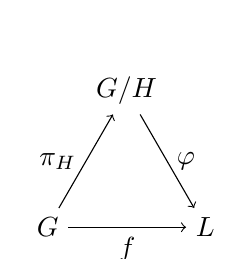
\begin{tikzpicture}
    % 定义三个节点的位置
    \node (G) at (0,0) {$G$};
    \node (L) at (2,0) {$L$};
    \node (GH) at (1,1.732) {$G/H$}; % 1.732 是根号3,用于等边三角形的高

    % 画箭头并添加标签
    \draw[->] (G) -- node[below] {$f$} (L); % G -> L,箭头下方写 f
    \draw[->] (G) -- node[left] {$\pi_H$} (GH); % G -> G/H,箭头左侧写 \pi_H
    \draw[->] (GH) -- node[right] {$\varphi$} (L); % G/H -> L,箭头右侧写 \varphi
\end{tikzpicture}

\(\varphi \circ \pi_H=f\)

example:
\begin{align}
    &(Z,+),n\in Z^{+}\\
    &f:Z\rightarrow Z_n\\
    &\forall a\in Z,f(a)=a\mod n,\text{这个是同态}\\
    &f:(Z,+)\rightarrow (Z_n,\oplus)\text{的同态}\\
    &ran(f)=Z_n,\text{suppose }a\in Z\\
    &ker(f)=\{a|a\in Z,f(a)=0\}=\{nq|q\in Z\}\\
    &G/H\overset{\varphi}{\rightarrow } Z_n\\
    &\varphi(aH)=a\%n,\text{是同构}
\end{align}


\subsection{有限循环群}
G是有限的循环群
\begin{align}
    &\exists g\in G,st. G=<g>=\{g^i|i\in Z\}\\
    &o(g)=n (g^n=I_G)\\
    &\forall i\in \{1,2,...,n-1\},g^i \neq I_G\\
    &\therefore G=\{i|i\in \{1,2,...,n-1\}\}
\end{align}

Pf:
\begin{align}
    &1.\text{suppose} d\in Z^{+},d|n,H=<g^d>,\\
    &\rightarrow H\leqslant G,|H|=\frac{n}{d}H=\{y|y\in G,y^{\frac{n}{d}}=I_G\}\\
    &2.H\leqslant G,\exists d\in Z^{+},H=<g^d>,d|n,st. H=<g^{d}>
\end{align}

有限循环群的子群,置换群

\begin{align}
    &G,H\leqslant G,\text{定义等价关系}\sim\\
    &\forall a,b\in G,a\sim b \leftrightarrow a^{-1}b\in H\leftrightarrow \exists h\in H,b=ah\\
    &1.(G,\sim)\text{为等价关系。用H为子群的特点}\\
    &2.a\in G,\{b|b\in G,a\sim b\}=\{a*h|h\in H\}=aH\\
    &3.a\sim b\rightarrow \forall g\in G,ga\sim gb
\end{align}

从陪集定义出发:
\begin{align}
    &aH=\{a*h|h\in H\}\\
    &I_H\in H\\
    &\therefore a\in aH\\
    &a,b\in G\text{下面几个等价}\\
    &1.a^{-1}b\in H\\
    &2.h\in aH\\
    &3.\exists a,h,b=ah\\
    &4.aH\cap bH\neq \varnothing\\
    &5.aH=bH
\end{align}

Pf:
\begin{align}
    &2\leftrightarrow 1 \leftrightarrow 3\\
    &b\in aH\rightarrow b=a*h,h\in aH\\
    &\leftrightarrow \exists h\in H,st. a^{-1}b=h\in H
    &\\
    &2\leftrightarrow 4\\
    &b\in aH,b\in bH,\therefore aH\cap bH\neq \varnothing\\
    &4\rightarrow 3\\
    &x\in aH\cap bH,\\
    &\because x\in aH,\exists h_1\in H,st. x=a*h_1\\
    &\because x\in bH,\exists h_2\in H,st. x=b*h_2\\
    &\therefore ah_1=b*h_2\\
    &\therefore a*h_1*h_2^{-1}=b\in aH\\
    &3\rightarrow 5\\
    &b=ah,h\in H,\text{Pf:}bH\subseteq aH\\
    &\forall x\in H,bx=ahx=a(hx)\\
    &\because H\leqslant G,h,x\in H,\therefore hx\in H\\
    &\therefore bx\in bH,bH\subseteq aH\\
    &\text{Pf:}aH\subseteq bH\\
    &b=ah,a=bh^{-1},h\in H\rightarrow h^{-1}\in H\\
    &\forall x\in H,ax=bh^{-1}x=b(h^{-1}x)\in bH\\
    &\therefore aH\subseteq bH\\
    &\therefore aH=bH
\end{align}

G为循环群,\(|G|\)=n,设\(G=<a>\),则
\begin{align}
    &1.\text{suppose} d \in Z^{+},d|n,H=<a^d>\\
    &\rightarrow H\leqslant G,|H|=\frac{n}{d},H=\{y|y\in G,y^{\frac{n}{d}}=I_G\}\\
    &2. \text{suppose} H\leqslant G,\exists d\in Z^{+},st.H=<a^d>\\
    &\{H|H\leqslant G\} \leftrightarrow \{d|d\in Z^{+},d|n\}\text{一一对应}
\end{align}

有几个子群:写出因子列出来。
\begin{align}
    &eg.n=6\\
    &<a^d>\rightleftarrows d\\
    & a, a^2, a^3, a^6=\{I_G\}
\end{align}

阶数的定义和性质:
\begin{align}
    &1.\forall m\in Z^{+},\exists m_0\in Z^{+},a^{m_0}=I_G\\
    &n=min\{m|a^m=I_G,m\in Z^{+}\}\\
    &\text{记} o(a)=n\\
    & a^i=I_G\leftrightarrow i|n\\
    & a^i=a^j\leftrightarrow i\equiv j \mod n\\
    &<a>=\{a^j|j=0,1,...,n-1\}\\
    &|<a>|=n=o(a)
\end{align}
Pf:
\begin{align}
    &1. o(a)=n;\text{断言} o(a^d)=\frac{n}{d}\\
    & (a^d)^{\frac{n}{d}}=I_G\\
    &Pf\\
    &i\in \{1,2,...,n-1\},\forall (a^d)^i=I_G\\
    & \leftrightarrow a^{id}=I_G\\
    &\leftrightarrow n|di\\
    &\leftrightarrow \frac{n}{d}|i\\
    &|<a^d>|=o(a^d)=\frac{n}{d}\\
    &2.H\text{也是一个循环群}\\
    & \exists b\in G,b=a^d,H=<b>=<a^d>\\
    &\\
    &\forall h\in H,h\in<a^d>,\exists i\in Z^{+},st. h=(a^d)^i=a^{di}\\
    &h^{\frac{n}{d}}=a^{ni}=I_G\\
    &\therefore \forall y\in G,\exists d,s.t. y^{\frac{n}{d}}=I_G,\exists i\in Z^{+},st. y=(a^d)^i=a^{di}\\
    &\because y\in <a>,\exists j\in Z,st. y=a^j\\
    & I_G=y^{\frac{n}{d}}=a^{j*\frac{n}{d}}\therefore n|j*\frac{n}{d}\\
    &\therefore d|j\\
    &y=a^j,H=<a^d>,\therefore y=(a^d)^\frac{j}{d}\in H
\end{align}

\begin{align}
    &\forall k\in Z,o(a^k)=\frac{n}{gcd(n,k)}\\
    &<a^k>=<a^{\frac{n}{gcd(n,k)}}>
\end{align}


\subsection{置换群}
设X是一个集合,
\begin{align}
    &Sym(X)=\{\sigma |\sigma X\rightarrow X,\sigma\text{是双射(置换)}\}\\
    &(Sym(X),\circ) \text{ is a group}\\
    &I_X:idx
    &\sigma \in Sym(X),\sigma^{-1}\in Sym(x)\\
    &(\sigma \circ \sigma^{-1}=\sigma^{-1}\circ \sigma =idx)\\
    &Sym(x)\text{是X上的对称群}\\
    &H\leqslant Sym(X),H\text{也是X上的置换群}\\
    & I_X\in H,\forall \sigma_1,\sigma_2\in H,\sigma_1\sigma_2\in H,\sigma_1^{-1}\in H\\
    &\forall a\in G,\text{def }L_a\in Sym(G),\text{(是双射)}\\
    &\forall b\in G,L_a(b)=a*b\text{左乘}\\
    &f:G \rightarrow Sym(G)\\
    &f(a)=L_a,f(ab)=L_a\circ L_b\text{f是单射,同态}
\end{align}

置换群的例子:
\begin{align}
    &X=\{1,2,...,n|n\in Z^{+}\}\\
    &Sym(X)=S_n\\
    & |S_n|=n!\\
    &eg. n=3\\
    &S_3=\{(1,2,3),(1,3,2),(2,1,3),(2,3,1),(3,1,2),(3,2,1)\}\\
    &\{\sigma |\sigma(i)\neq i\forall 1\leqslant i\leqslant n\}=C_n\\
    &\frac{|C_n|}{n!}=\Sigma_{i=0,n} \frac{(-1)^n}{i!}
\end{align}

\begin{align}
    &Sym(X) \text{对换i,j},i\in X,j\in X,i\neq j,\sigma(i)=j,\sigma(j)=i\\
    &\text{三轮换}
\end{align}

计算题
\begin{align}
    &S_5,\\
    &\alpha =\begin{pmatrix}
        1&2& 3& 4& 5\\
        2& 3 &1 &5& 4
        \end{pmatrix}\\
    &\beta =\begin{pmatrix}
        1&2& 3& 4& 5\\
        1&3&4&5&2
    \end{pmatrix}\\
    &\alpha\circ \beta=\alpha(\beta)=\begin{pmatrix}
        1&2& 3& 4& 5\\
        2&1&5&4&3
    \end{pmatrix}\\
    &\beta\circ \alpha=\beta(\alpha)=\begin{pmatrix}
        1&2& 3& 4& 5\\
        3&4&1&2&5
    \end{pmatrix}\\
    &\alpha^{-1}=\begin{pmatrix}
        1&2& 3& 4& 5\\
       3& 1 &2 &5& 4
    \end{pmatrix}\\
\end{align}

三次对称群
\begin{align}
    &Sym(X)=\{\sigma |\sigma :X\rightarrow X\text{双射}\}\\
    &S_3=\{(1,2,3),(1,3,2),(2,1,3),(2,3,1),(3,1,2),(3,2,1)\}\\
    &\text{第一个非交换群。一个六阶非交换群同构于}S_3\\
    &\text{一阶ok;二阶{e,a},三阶循环群,四阶循环或者klein,五阶素数循环群}\\
    &\sigma=(a_1,a_2,a_3,...,a_m):\sigma(a_1)=a_2,...,\sigma(a_m)=a_1\\
    & \text{幺元:}\begin{pmatrix}
        1&2&3\\
        1&2&3
    \end{pmatrix}\\
    &\text{令}\tau (1,2,3)\\
    &\tau ^2=(1,3,2)\\
    &\tau ^3=I_{S_3}\\
    &\\
    &H=<\tau>=\{(1,2,3),(1,3,2),idx\} \lhd S_3\\
    & \eta =(1,2)\\
    &\eta \tau \eta^{-1}=\tau^2\\
    &S_3=<\{\eta,\tau\}>\\
    &|H|=3(\tau^i)\\
    &|\eta H|=3(\eta\tau^i)(\eta\notin H)\\
    &\therefore H\cup \eta H=S_3\\
    &\text{计算题:}
    &\eta \tau \neq \tau \eta\\
    &\eta \tau \eta^{-1}=\tau^2\\
    &\tau \eta \tau\eta^{-1}\tau^2=\tau \tau \tau^2=\tau\\
    &S_3\text{'s subgroup}:\\
    &1.\{id\}\\
    &2.\{id,(1,2)\},\{id,(2,3)\},\{id,(1,3)\}\\
    &3. \{id,(1,2,3),(1,3,2)\}\text{only one}\\
    &6. S_3
\end{align}

\begin{align}
    &(a_1,...,a_m),(b_1,...,b_k),a_i\neq b_j,\text{两个轮换不相交,没有公共变动元素}\\
    &\rightarrow (a_1,...,a_m)(b_1,...,b_k)=(b_1,...,b_k)(a_1,...,a_m)\\
    &eg.S_7:\\
    &(1,2,3)=\begin{pmatrix}
        1&2&3&4&5&6&7\\
        2&3&1&5&4&6&7
    \end{pmatrix}\\
    &(4,5,6)=\begin{pmatrix}
        1&2&3&4&5&6&7\\
        1&2&3&5&6&4&7
    \end{pmatrix}\\
    &(1,2,3)(4,5,6)=\begin{pmatrix}
        1&2&3&4&5&6&7\\
        2&3&1&5&6&4&7
    \end{pmatrix}=(4,5,6)(1,2,3)\\
    &\forall \sigma \in Sym(X),M(\sigma)=\{x|x\in X,\sigma(x)\neq x\}\\
    &\sigma_1,\sigma_2\in Sym(X),if. M(\sigma_1)\cap M(\sigma_2)=\varnothing\\
    &\sigma_1\sigma_2=\sigma_2\sigma_1
\end{align}

Thm:Sn中任何一个置换可以写成两两不相交的轮换的乘积(复合),且在不计次序的情况下分解唯一(不考证明)\\

\begin{align}
    &Sym(X),\sigma \in Sym(X),\forall x\in X,\text{x所在的轮换}\\
    & \exists only. k\in Z^{+},st.\sigma(x)^k=x,\forall i\in\{1,2,...,k-1\},\sigma(x)^i\neq x\\
    &\text{这个轮换写成:(也是分解式之一)}(x,\sigma(x),\sigma(\sigma(x)),...,(\sigma^{k-1}(x)))
\end{align}

def:
\begin{align}
    &\sigma \in Sym(X)\\
    &def:(X,\sim)\\
    &i\sim j\leftrightarrow \exists l\in Z,st. j=\sigma^l(i)\\
    &\rightarrow  \text{ 每个轮换元素在一个等价类里面}\\
    &(\text{轮换ok,不相交的对换不一定,可以相交的对换ok})
\end{align}

eg:
\begin{align}
    &(1,2,3)=(1,2)(2,3)\\
    &(a_1,...,a_m)=(a_1,a_2)(a_2,a_3)...(a_{m-1},a_m)\\
    &\text{置换可以写成对换的乘积}\\
    &S_n\text{中有}C_n^2=\frac{你(n-1}{2}\text{个轮换}\\
    &\text{命题} S_n\text{can be produced by:}\\
    &(1,2),(2,3),(3,4),...,(n-1,n)\\
    &eg. (1,3)=(1,2)(2,3)(1,2)\\
    &(1,4)=(1,3)(3,4)(1,3)=(1,2)(2,3)(1,2)(3,4)(1,2)(2,3)(1,2)\\
    &(i,j)(j,k)(i,j)=(i,k)\\
    &\text{Statement:Sn can be produced by two elements}\\
    &(1,2)(1,2,..,n) \\
    &(1,2,...,n)(i-1,i)(1,...,n)^{-1}=(i,i+1)\text{min }\\
    &\text{奇/偶数置换}\\
    &S_n: \{1,2,...,n\}\text{的所有置换}\\
    &\sigma=(a_1,b_1)...(a_m,b_m)=(c_1,d_1)...(c_k,d_k)\\
    &\therefore m\equiv k \mod 2
\end{align}

下面证明以上命题

\begin{align}
    &I_n=\begin{pmatrix}
        1&0&0\\
        0&1&0\\
        0&0&1
    \end{pmatrix}\\
    &\text{三阶单位阵有六种变换形式,对应三阶置换群的6个元素}、、
    &\sigma\in S_n,\text{如下定义n阶矩阵}A\\
    &A_{ij}=\left\{
        \begin{aligned}
        &1 \text{ if i=}\sigma(j) \\
        &0 \text{ if i}\neq\sigma(j) \\
        \end{aligned}
    \right.\\
    &1.\forall \sigma,A(\sigma(i),j)=1\\
    &2. \forall 1\leqslant i,j\leqslant n,i\neq \sigma(j),A(i,j)=0\\
    &\text{in fact:define a f},S_n\rightarrow M_n,\text{由}f(\sigma)=\sigma\text{确定的置换矩阵}\\
    &\text{f是同态}\\
    & f(\sigma \tau)=f(\sigma)* f(\tau)\text{矩阵乘法(不考证明)}\\
    &Pf:\\
    &A=f(\sigma),B=f(\tau),C=f(\sigma*\tau)\\
    &C(i,j)=\left\{
        \begin{aligned}
        &1 \text{ if i}=\sigma \circ \tau(j)=\sigma(\tau(j)) \\
        &0 \text{ if i}\neq\sigma(\tau(j)) \\
        \end{aligned}
    \right.\\
    &\text{we want to prove C=AB}\\
    &AB(i,j)=\Sigma_{k=1}^n A(i,k)*B(k,j)\\
    &i=\sigma(k),k=\tau(j)\rightarrow i=\sigma(\tau(j))\\
    &AB(i,j)=\Sigma_{k=1}^n A(i,\tau(j))*B(\tau(j),j)\\
    &\text{在}i=\sigma(\tau(j))\text{才等于1.C同理}
    &\\
    &\text{suppose} \sigma=(a_1,b_1)...(a_m,b_m)\\
    &f(\sigma)=f((a_1,b_1))...f(a_m,b_m))\\
    &det(f(\sigma))=det(f((a_1,b_1))...f((a_m,b_m)))\\
    &\text{一个对换的行列式是-1}\\
    &(-1)^{m}=(-1)^{k},ok
\end{align}

逆序对
\begin{align}
    &\sigma \in S_n\\
    &T(\sigma)=\{(i,j)|1\leqslant i<j\leqslant n,\sigma(i)>\sigma(j)\}\\
    &=\sigma\text{的全部逆序对}\\
    &|T(\sigma\circ \tau)|=|T(\sigma)|+|T(\tau)|(mod 2)\\
    &(2|m+k)\\
    &\\
    &\text{suppose } A_n=\{\sigma|\sigma \in S_n,\sigma\text{是偶置换}\}\\
    &(A_n)
    &(i,j)(i,j)=id\\
    &\forall \sigma\in A_n,(1,2)\sigma\text{是奇置换}\\
    &\tau\in S_n-A_n,(1,2)\tau\text{是偶置换}\\
    &S_n=A_n\cup (1,2)A_n\\
    &\therefore|A_n|=\frac{n!}{2}\\
    &\sigma\text{可写为不相交的轮换的乘积}\\
    &\sigma=\tau_1\tau_2...\tau_{k},\text{阶数为}d_1,...,d_k\\
    &o(\sigma)=lcm(d_1,...,d_k)\\
    &Pf:\\
    &\tau_1\tau_2=\tau_2\tau_1\\
    &\sigma ^m=\tau_1^m\tau_2^m...\tau_k^m\\
    &\sigma^m=id\leftrightarrow \forall i,\tau_i^m=id\\
    &\leftrightarrow \forall i, d_i|m\\
    &\leftrightarrow lcm(d_1,...,d_k)|m\\
    &\text{考察题型:求置换的乘积;不相交轮换分解;置换的阶}
\end{align}

(如果 \(\sigma^m = id\),则 \(\sigma\) 的 \(m\) 次幂必须将每个元素映射回它自身。由于 \(\sigma\) 是不相交轮换 \(\tau_1, \tau_2, \ldots, \tau_k\) 的乘积,每个 \(\tau_i\) 也必须将每个元素映射回它自身,即 \(\tau_i^m = id\)。)

\subsection{Sylow 定理}
\begin{align}
    &G\text{是有限的群}\\
    &H\leqslant G,H\text{是G的子群}\\
    &d||G|\\
    &\text{有d阶子群吗?}\\
    &A_4\text{没有六阶子群}  
\end{align}

群论学家:\\
伽罗瓦\\
阿贝尔\\
Sylow\\
Burnside\\
Frobenius\\
Kurosh\\
Wielandt\\
Huppet\\
段学复\\
张远达


DEF:
\begin{align}
    &G\text{是有限群}\\
    &|G|=n,p\text{ is prime}\\
    &\text{suppose} p^k|n,p^{k+1}\nmid n\\
    &1.\text{if } |H|\text{是p的幂次,H是G的p-子群}\\
    &2.if.|H|=p^k,H\text{是G的Sylow-p子群}\\
    &|H|\text{是p-子群,}|H|=p^l,\therefore l\leqslant k\\
    &\\
    &G,A\subseteq G,gAg^{-1}=\{gag^{-1}|\forall a\in A\}
    & def:f:G\rightarrow G\\
    &\forall a\in G,f(a)=gag^{-1}\\
    &\text{f是G到自身的群同构(双射+同态)},f^{-1}=g^{-1}ag\\
    &f:\text{由g诱导的内自同构(可能会考)}
\end{align}

Sylow定理
\begin{align}
    &G\text{是有限群},|G|=n,p.prime\\
    &\therefore\\
    &1.G\text{有Sylow-p子群}\\
    &|\{H|H\text{是Sylow-p子群}\}|\equiv 1(mod p)\\
    &2.H,K\text{are two Sylow-p子群}\\
    &\rightarrow \exists g\in G,K=gHg^{-1}\\
    &3.A \text{是G的p-子群},\exists H \text{是G的Sylow-p子群},st. A\subseteq H
\end{align}

Stronger:
\begin{align}
    &1':p^l|n,\rightarrow\\
    &|\{A|A\leqslant G,|A|=p^l\}|\equiv 1(mod p)\\
    &\text{证明大致思路:分成等价类,每个等价类里面要么没有子群要么只有一个}
\end{align}

Statement:
\begin{align}
    &\text{G是偶数阶群}\\
    &\therefore |\{a|a\in G,a^2=I_G\}|\equiv 0(mod 2)\\
    &=\{I_G\}\cup \{\text{G中二阶元}\}\\
    &\rightarrow \text{二阶子群的个数是奇数}
\end{align}

\begin{align}
    &\text{定义等价关系}\\
    &\forall a,b\in G,a\sim b \leftrightarrow a=b/a=b^{-1}a\\
    &\forall a\in G,\text{a在\(\sim\)下的等价类}:\{b|b\in G,a\sim b\}=\{a,a^{-1}\}\\
    &|\{a,a^-1\}|=\left\{
        \begin{aligned}
        &1,a^2=I_G\\
        &2,a^2\neq I_G
        \end{aligned}
    \right.\\
    &\text{记T是G在\(\sim\)下的等价类的集合}\\
    &|G|=\Sigma_{A\in T}|A|=\Sigma_{A\in T,|A|=1}|A|+2\Sigma_{A\in T,|A|=2}|A|\\
    &=|\{a|a^2=I_G\}|+2|\{a|a^2\neq I_G\}|\\
    &\text{G是偶数阶群}\\
    &\therefore |\{a|a^2=I_G\}|\equiv 0(mod 2)\\
    &\text{这一段也可以像下面这么写:}\\
    & \text{记}A_1,...,A_m\text{是全体等价类}\\
    &|A_1|=...=|A_l|=1,|A_{l+1}|=...=|A_m|=2\\
    &|G|=l+2(m-l)\\
    &ok
\end{align}

\begin{align}
    &\text{G为n阶群,\(d|n\),考察G中有无d阶子群}\\
    &\text{记T}=\{A|A\subseteq G,|A|=d\}\\
    &\text{定义等价关系}\\
    &A\sim B \leftrightarrow \exists g\in G,st. B=gA=\{ga|a\in A\}\\
    &\forall A\subseteq G,|A|=d,\text{A所在的等价类}:\{B|B\subseteq G,|B|=d,A\sim B\}=\{gA|g\in G\}(\text{这里不要求子群})\\
    &\\
    &G/H=\{gH|g\in G\},H\leqslant G\\
    &for.A\leqslant G,\text{记}[A]=\{gA|g\in G\},\rightarrow\\
    &1.if[A]\text{中有子群,则有且只有一个,},|[A]|=\frac{n}{d}\\
    &2.if_not_ |[A]|=\frac{n}{d}*w,w\geqslant 2,w|d\\
    &\text{记}L_1,...,L_m\text{是全体等价类}\\
    &L_1,...,L_k\text{have subgroup},L_{k+1},...,L_m\text{have no subgroup}\\
    &\rightarrow \text{have k d阶subgroups }
\end{align}

\begin{align}
    &\text{G is a finite group, } d \mid n, \text{ and } H \leq G,\\
    & \text{ we want to determine whether } ,p^l||G|,\\
    &\text{the number of the subgroups of order }p^l\\
    &\text{ is odd.(考试只需证明有就可以,不要求证明奇数)}\\
    &Statement:\\
    &\text{G is a finite group,},d\mid n,d\geqslant 2,\text{the number of the subgroups of order d is k}\\
    &\text{\textcircled{1}} \exists d,\text{有一些d的因子}\geqslant 2,(w_i|d),st.\\
    &((n-1),d-1)=k+w_1+w_2+...+w_s\\
    &\text{\textcircled{2}} \text{p is a prime number},d=p^l\rightarrow k\geqslant 1\\
    &\text{\textcircled{3}} .for \text{\textcircled{2}},k\equiv 1(mod p)\\
    &Pf:\\
    &\text{\textcircled{1}}\rightarrow \text{\textcircled{2}},\text{\textcircled{3}}\\
    &\text{代入}d=p^l,\therefore((n-1),p^l-1)=k+w_1+w_2+...+w_s\\
    &\forall 1\leqslant i\leqslant s,w_i|p^l\\
    &\therefore w_i=p^t(t\leqslant l,t\neq 0)\\
    &\therefore p|w_i\\
    &\therefore ((n-1),p^l-1)\equiv k (mod p)(\text{考试考到这里})\\
    &\text{p is a prime number},p^l|n,\therefore((n-1),p^l-1)\equiv 1\equiv k(mod p)
\end{align}

Pf刚刚的几个命题:
\begin{align}
    &T=\{A|A\leqslant G,|A|=d\},\sim:\\
    &A\sim B \leftrightarrow \exists g\in G,st. B=gA=\{ga|a\in A\}\\
    &\forall A\subseteq G,|A|=d,\text{A所在的等价类}:[A]=\{gA|g\in G\}\\
    &\text{and }1.if_[A] \text{中有子群,则有且只有一个,},|[A]|=\frac{n}{d}\\
    &2.if_not_ |[A]|=\frac{n}{d}*w,w\geqslant 2,w|d\\
    &\text{这里还没证明,证明见后面}\\
    &\text{记}L_1,...,L_m\text{是全体等价类}\\
    &\text{G中d阶子群个数为k,分布在k个等价类里面,不妨设是}L_1,...,L_k\\
    &\therefore |L_1|=...=|L_k|=\frac{n}{d}\\
    & \forall k+1\leqslant j\leqslant m,|L_j|=\frac{n}{d}*w_j,w_j\geqslant 2,w_j|d\\
    &|T|=\frac{n}{d}*k+\Sigma_{j=k+1}^m \frac{n}{d}*w_j\\
    &|T|=C_n^d=\frac{n}{d}C_{n-1}^{d-1},\therefore ok 
\end{align}

作用:
定义:幺半群在集合上的作用
\begin{align}
    &\forall g\in X,g\rightarrow X=\rightarrow (g,X)\\
    &1.\forall g,h\in G,x\in H,(gh)\rightarrow x=g\rightarrow (h\rightarrow x)\\
    &2.\forall x\in H,I_G\rightarrow x=x\\
    &\text{称X是幺半群G上的作用}\\
    &\\
    &A\sim B:\exists g\in G,st. B=gA=\{ga|a\in A\},\text{群在子集上的作用}\\
    &\text{定义:}g\rightarrow A=gA.\\
    &I_G\rightarrow A=A\\
    &(gh)\rightarrow A=(gh)A\\
    &eg.\\
    &\text{X is a set,G=Sym(X) },\sigma\rightarrow x=\sigma(x)\\
    &id\rightarrow x=x\\
    &(\sigma \circ \tau)\rightarrow x=\sigma(\tau(x))
\end{align}

共轭作用
\begin{align}
    &g\rightarrow X=gXg^{-1}\\
    &1.I_G\rightarrow X=X\\
    &2.(gh)\rightarrow X=(gh)X(g^{-1}h^{-1})=g\rightarrow(h\rightarrow x)\\
    &\text{类比}:G,X=2^G.H\leqslant G,and_H\lhd G\rightleftarrows \forall g\in G,gHg^{-1}=H\leftrightarrow \forall g \in G,g\rightarrow H=H\\
    &eg.GL_2(R)=\{\begin{pmatrix}
        a&b\\
        c&d
    \end{pmatrix}|a,b,c,d\in R,\text{矩阵可逆}\}\\
    &X\text{是2元列向量}\\
    &def  A\rightarrow \beta=A\beta\\
    &\alpha ,\beta\in X,\alpha ,\beta \neq 0;\\
    &\exists A\in G,st. \beta=A\alpha.\\
    &\alpha =(1,0)^T,\beta=(c,d)^T,\\
    &\text{令}A=\begin{pmatrix}
        c&*\\
        d&*
    \end{pmatrix}\\
    &(\text{(**)和(c,d)线性无关即可。这样A可逆})\\
    &\rightarrow A\alpha=\beta
\end{align}

群作用和等价关系:
\begin{align}
    &x\sim y\leftrightarrow \exists g\in G,st. y=g\rightarrow x\\
    &\text{自反}I_G\rightarrow x=x,x\sim x\\
    &\text{对称}x \sim y\leftrightarrow y=g\rightarrow x\leftrightarrow x=g^{-1}\rightarrow y \\
    &\text{传递}x\sim y,y\sim z\rightarrow y=g\rightarrow x,z=h\rightarrow y\Rightarrow z=(hg)\rightarrow x\rightarrow x\sim z
\end{align}

群作用的轨道公式:
\begin{align}
    &\text{if X is finite,suppose }U_1,...,U_m\text{是}(X,\sim)\text{的两两不同的等价类}\\
    &\therefore |U_1|+...+|U_m|=|X|\\
    &\forall x\in X,\text{x所在的等价类}:\{y|y\in X,x\sim y\}={g\rightarrow x|g\in G}\text{是X上的一个轨道}\\
    &\text{记为}G_x/orbit(x)/G(x),\text{称为x在G作用下的轨道}\\
    &stab(x)=\{g|g\in G,g\rightarrow x=x\}\text{作用在G上不变,稳定化子}
\end{align}

Statement:
\begin{align}
    &\text{G依作用→作用在X上,}x \in X\\
    &\text{记}G_x=\{g\rightarrow x|g\in G\},H=stab(x)=\{g|g\in G,g\rightarrow x=x\}\\
    &\rightarrow:\\
    &1.H\leqslant G\\
    &2.\forall a,b\in G, a\rightarrow x=b\rightarrow x\leftrightarrow a^{-1}b\in H\leftrightarrow aH=bH\\
    &3. \phi:G/H\rightarrow G_x\\
    &def:\forall a\in G,\phi(aH)=a\rightarrow x\\
    &\text{那么这个是合理定义的(如果aH=bH,但是作用下的结果不相同,就不合理)}\\
    &4.\text{如果G,X是有限的},|G_x|=\frac{|G|}{|H|}=|G/H|\\
    &Pf:\\
    &1.I_G\rightarrow x=x,\therefore I_G\in H\\
    &a,b\in H,a\rightarrow x=b\rightarrow x=x,(ab)\rightarrow x=x,\therefore ab\in H\\
    &a^{-1}\rightarrow x=a^{-1}\rightarrow(a\rightarrow x)=x\rightarrow a^{-1}\in H\\
    &ok.\\
    &2. if. a\rightarrow x=b\rightarrow x\\
    &(a^{-1}b)\rightarrow x=a\rightarrow (a\rightarrow x)=x.\\
    &if.(a^{-1}b)\rightarrow x =x,\rightarrow a\rightarrow x=a\rightarrow((a^{-1}b)\rightarrow x)=b\rightarrow x\\
    &\therefore a\rightarrow x=b\rightarrow x\leftrightarrow a^{-1}b\in H\leftrightarrow aH=bH(\text{这个是陪集的定义})\\
    &3. \phi:G/H\rightarrow G_x\\
    &\text{由2,}aH=bH\rightarrow a\rightarrow x=b\rightarrow x\\
    &\therefore \phi(aH)=\phi(bH)\rightarrow a\rightarrow x=b\rightarrow x\rightarrow aH=bH\text{所以是单射}\\
    &ran(\phi)=G_x,\forall a\in G,a\rightarrow x=\phi(aH)\in ran(\phi)\\
    &(\phi':G\rightarrow G_x)\\
    &(\phi'(a)=a\rightarrow x)\\
    &4.G_x,G/H\text{一一对应(由于phi)}
\end{align}

Statement:
\begin{align}
    &\text{有限群G按照→作用在有限集X上,}U_1,...,U_m\text{两两不同的轨道}\\
    &\text{记} U_i=G_{x_i}.
    &\rightarrow |X|=\Sigma_{i=1}^m \frac{|G|}{|stab(X_i)|}\\
    &Pf:\\
    &\forall i,U_i=G_{x_i}\\
    &|U_i|=|G_{x_i}|=\frac{|G|}{|stab(x_i)|}\text{从上面那个结论推出来的}
\end{align}

不动点定理

\begin{align}
    &g\rightarrow x=x:\text{x是不动点}\\
    &\leftrightarrow G_x=\{x\}\leftrightarrow stab(x)=G\\
    &\text{G共轭作用在G上,}:g\rightarrow x=gxg^{-1}\\
    &x\in G,\text{x是共轭作用下的不动点}\leftrightarrow \forall g\in G,g\rightarrow x=x\leftrightarrow \forall g\in G,gxg^{-1}=x\leftrightarrow gx=xg\\
    &Z(G)=\{x|x\in G,\forall g\in G,gx=xg\}:\text{G的中心}\\
    &eg.\text{对二阶可逆实矩阵},Z(G)=\{\begin{pmatrix}
        a&0\\
        0&a
    \end{pmatrix}|a\neq 0\}\\
    &\text{n阶:}aI_n
\end{align}

Statement:
\begin{align}
    &\text{p是素数,}|G|=p^k\\
    & G,\rightarrow,Y:\text{全体不动点}\\
    &\rightarrow|X|=|Y|(mod p)\\
    &if. p\nmid |X|,\text{则有不动点}\\
    &Pf:\\
    &U_1,...,U_m\text{all orbits}\\
    &U_i=G_{x_i}\\
    &\text{不妨设前k个有一个元素,其他的至少两个}\\
    &i=1\sim k:|U_i|=\frac{|G|}{|stab(x_i)|}=1\\
    &i=k+1\sim n:|U_i|=\frac{|G|}{|stab(x_i)|}\geqslant 2\\
    &|stab(x_i)|||G|\text{根据前面那个除法式子}\\
    &\because |U_i|\text{是p的幂次},|U_i|\geqslant 2\\
    &\therefore p||U_i|\\
    &\therefore |X|\equiv k(mod p)\\
    &\therefore |Y|=k\text{设 Y 是 X 中的全体不动点,那么 Y 中的元素对应的轨道大小都是 1}
\end{align}

Statement:
\begin{align}
    &\text{G is finite,p is prime},|A|=p^k,H\leqslant G,p\nmid\frac{|G|}{|H|},\\
    &\therefore \exists g\in G,st. A\subseteq gHg^{-1}\\
    &Pf:\\
    &\text{考虑}G/H,A\text{依左乘作用在G/H上}\forall a\in A,\forall g \in G,a\rightarrow(gH)=agH\\
    &|A|\text{是p的幂次},p\nmid |G/H|(\text{根据上一个命题构造的A})\\
    &\rightarrow \text{有不动点}\\
    &\text{取}g\in G,st, gH\text{是不动点},\forall a\in A,a\rightarrow(gH)=gH,\\
    &agH=gH\rightarrow ag\in gH\rightarrow a\in gHg^{-1}\rightarrow ok.
\end{align}

Sylow定理第二部分:

\begin{align}
    &\text{G is finite.p is prime.},p^k||G|,p^{k+1}\nmid |G|\\
    &(p^k  \text {是 G 的阶数中 p 的最高幂次因子},|H|=p^k)\\
    &\therefore \\
    &1.H,K\text{are two Sylow-p子群},\exists g\in G,K=gHg^{-1}\\
    &2.\text{A is a p-subgroup},\exists\text{a Sylow-p subgroup H },st.A\subseteq H.\\
    &Pf:\\
    &1.K \text{is p-subgroup},p\nmid |G|/|H|\\
    &(\text{根据前面讨论的不动点定理,H 在 G 的共轭作用下存在不动点})\\
    &\exists g\in G,st.K\subseteq gHg^{-1}\\
    &\text{但是}|K|=p^k,|H|=|gHg^{-1}|=p^k,\therefore ok.\\
    &2.\text{取一个G的Sylow子群L},a\text{is a p-subgroup},p\nmid |G|/|L|\\
    & \therefore \exists g\in G,st. A\subseteq gLg^{-1}=H
\end{align}

\begin{align}
    &\text{另外:第一部分里面有一个}C_{n-1}^{p^l-1}\equiv 1(mod p):\\
    &C_n^m,\text{p进制下},n=n_k,...,n_0;m=m_k,...,m_0\\
    &C_n^m=\Pi C_{n_i}^{m_i}(mod p)\\
    &p^l:\text{1后面l个零}\\
    &p^l-1:\text{l个(p-1)}\\
    &n-1:n_k,...,n_1(n_0-1)\\
    &C_{n_i}^{p-1},\text{在ni大于等于p-1的时候才不等于零},n_i=p-1,=1\\
    &n=k*p^l,\therefore n-1:(k-1)(p-1)...(p-1)\\
    &C_{n-1}^{p^l-1}=C_{k-1}^0*1*...1\equiv 1(mod p)
\end{align}


\section{RING!}
\subsection{def}
\begin{align}
    &(R,+,*)\text{is a ring}\\
    &1.(R,+)\text{是交换群,幺元记为0}\\
    &2.(R,*)\text{is a monoid,幺元记为}I_R\\
    &3.\forall a,b,c\in R,a(b+c)=ab+ac,(a+b)c=ac+bc\\
    &if. ab=ba,\text{是交换环}
\end{align}

example:

\begin{align}
    &1.(M_n(R),+,*)\\
    &2.n\in Z^+,(\{0,1,...,n-1\},\oplus ,\otimes )\\
    &3.\text{实数序列}(a_0,a_1,...,a_n,...)\\
    &(a_0,a_1,...,a_n,...)+(b_0,b_1,...,b_n,...)=(a_0+b_0,a_1+b_1,...,a_n)\\
    &text{multiply:}\\
    &c_0=a_0b_0\\
    &c_1=a_0b_1+a_1b_0\\
    &c_2=a_0b_2+a_1b_1+a_2b_0\\
    &...\\
    &c_n=a_0b_n+a_1b_{n-1}+...+a_{n-1}b_1+a_nb_0\\
    &(\Sigma a_ix^2)+(\Sigma b_ix^2)=(\Sigma (a_i+b_i)x^2)\\
    &(\Sigma a_ix^2)*(\Sigma b_ix^2)(\Sigma \Sigma _{i+j=n} a_i+b_j x^n)\\
    &4.Z_2^n=\{0,1\}^n,\text{长度为n的0,1序列}\\
    & (Z_2^n,\oplus),(0,0,...,0)\\
    &(Z_2^n,\otimes),(1,1,..,1)\\
    &5. \text{集合X和环的关系:}\\
    &\text{ for two sets,A and B}\\
    &A\oplus B=(A-B)\cup (B-A)=A\cup B-A\cap B\\
    &P(X)=\{A|A\subseteq X\},\\
    &(P(X),\oplus,\cap)\text{is a ring}\\
    &\text{序列}(a_1,...,a_n)\rightarrow A=\{i|1\leqslant i\leqslant n,a_i=1\}\in P(X)\\
    &\phi:Z_2^n\rightarrow P(X)\\
    &\phi (a_1,...,a_n)=\{i|1\leqslant i\leqslant n,a_i=1\}\\
    &\phi(\alpha)=A,\phi(\beta)=B\\
    &\phi(\alpha \oplus \beta)=A\oplus B\\
    &\phi(\alpha  \beta)=A\cap B\\
\end{align}

群环:\\
\begin{align}
    &\text{G is a finite group,C is complex}\\
    &C^G: f: G\rightarrow C\\
    &(C^G,+,*):\\
    &f,g\in C^G,(f+g)(a)=f(a)+g(a),\\
    &*f*g (a)=\Sigma_{b\in G}f(b)g(b^{-1}a)\\
    &=\Sigma _{(b,c)\in G*G,bc=a} f(b)g(c)\\
\end{align}

四元数环\\
\begin{align}
    &R=\{\begin{pmatrix}
        \alpha & \beta\\
        -\beta & \alpha
    \end{pmatrix} |\alpha,\beta \in C\}\\
    &\\
    &I_2=\begin{pmatrix}
        1&0\\
        0&1
    \end{pmatrix}\\
    &i=\begin{pmatrix}
        \sqrt{-1}&0\\
        0&\sqrt{-1}
    \end{pmatrix}\\
    &j=\begin{pmatrix}
        0&1\\
        -1&0
    \end{pmatrix}\\
    &k=\begin{pmatrix}
        0&\sqrt{-1}\\
        -\sqrt{-1}&0
    \end{pmatrix}\\
    &i^2=j^2=k^2=I_2,ij=k,ji=-k\\
    &a+bi+cj+dk
\end{align}

mod剩余类环:
\begin{align}
    &\{Z_n,\oplus,\otimes\}
\end{align}

\begin{align}
    &\text{if }(R,+,*)\text{ is a ring}\\
    &1.a0=0a=0\\
    &2.-(ab)=(-a)b=a(-b)\\
    &Pf:\\
    &1. a0=a(0+0)=a0+a0\rightarrow a0=0,\\
    &0a=(0+a)0=a0+a0\rightarrow 0a=0\\
    &2.0=a0=a(b+(-b))\rightarrow ok
\end{align}


\begin{align}
    &(R,+,*)\text{is a ring}\\
    &(R,+)\text{是交换群}\\
    &(R,*)\text{is a semigroup,if 有幺元,记作}I_R\\
    &\text{if ab=ba,是交换环}
\end{align}


\begin{align}
    &(F,+,*)\text{是域:}\\
    &1.(F,+,*)\text{是交换环,有乘法幺元} I_F\\
    &2.\forall a,b\in F,a,b\neq 0,ab^{-1}\in F\\
    &\text{另外一种写法:}\\
    &1.(F,+)\text{是交换群,幺元是0}\\
    &2.(F,*)\text{是交换幺半群,或者:}(F-{0},*)\text{是群}\\
    &3.\text{分配律}a(b+c)=ab+ac
\end{align}

\begin{align}
    &\text{field:}Q,R,C.\text{Z is not a field}\\
    &\text{other examples:}\\
    &K=\{a+b\sqrt{2}| a,b\in Q\}\\
    &(K,+,*)\\
    &1.\text{交换环:}\\
    &a. \text{(K,+)是交换群}\\
    &\text{封闭,结合,有幺元,有逆元}\\
    &\text{逆元}:-a-b\sqrt{2}\\
    &\text{交换群:}(a+b\sqrt{2})+(c+d\sqrt{2})=(c+d\sqrt{2})+(a+b\sqrt{2})\\
    &b.(K,*)\text{是半群或者幺半群都可以}\\
    &\text{封闭,结合(幺元是1)}\\
    &c. \text{分配律}\\
    &a(b+c)=ab+ac\\
    &(a+b)c=ac+bc\\
    &\text{交换环}\\
    &(a+b\sqrt{2})(c+d\sqrt{2})=(c+d\sqrt{2})(a+b\sqrt{2})\\
    & \\
    & I_K=1\\
    &\forall a+b\sqrt{2}\in K,\text{有逆元} \frac{a}{a^2-2b^2}-\frac{b}{a^2-2b^2}*\sqrt{2}
\end{align}

\begin{align}
    &L=\{a+b\sqrt[3]{2}+d\sqrt[3]{4}|a,b,c\in Q\}\text{类似}\\
    &a+b\pi\text{是环不是域}\\
    &\{\{0,1,...,n-1\},\oplus,\otimes\}\text{是交换环不是域}\\
    &Z_6: 2\otimes 3=0\\
    &if 2\otimes x=0\rightarrow 2x\equiv 1(mod 6),no \text{3也没有乘法逆元}\\
    &Z_5\text{is a field}
\end{align}

Statement:
\begin{align}
    &(Z_n,\oplus,\otimes)\text{is a field}\leftrightarrow \text{n is a prime}
\end{align}

\begin{align}
    &\text{分式域:}\\
    &R_{[x]}=\{a_0+...+a_n x^n|n\in N,\forall a_i\in R\}\\
    &\text{乘法幺元是1,逆元没有,所以:}
    &R(x)=\{\frac{f}{g}|f,g\in R_{[x]},g\neq 0\}\\
    &\text{这样有逆元了}
\end{align}

\subsection{环作用(不要求)}

\begin{align}
    &\text{凯莱定理:半群也可以}\\
    &R^n:\text{R上的向量空间}\\
    &1. (\alpha+\beta)+\gamma=\alpha+(\beta+\gamma)\\
    &2. \overset{\rightarrow}{0}\in R^n,\overset{\rightarrow}{a}+\overset{\rightarrow}{0}=\overset{\rightarrow}{0}+\overset{\rightarrow}{a}=\overset{\rightarrow}{a}\\
    &3.\forall \alpha \in R^n,\alpha+(-\alpha)=\overset{\rightarrow}{0}\\
    &4.\alpha +\beta=\beta+\alpha\\
    &5.(ab)\alpha=a(b\alpha)\\
    &6.1*\alpha=\alpha\\
    &7.(a+b)\alpha=a\alpha+b\alpha\\
    &8. a(\alpha+\beta)=a\alpha +a\beta \\
    &\text{一到四是加法作用下的交换群,5,6是作用,7,8是分配律}
\end{align}

\begin{align}
    &(R,+,*)\text{is a ring,有幺元},(M,+)\text{ is a Abel group}\\
    &\rightarrow :\forall a\in R,x\in M,a\rightarrow x=ax\\
    &if:1.\forall a,b\in R,\forall x\in M,a\rightarrow (b\rightarrow x)=(ab)\rightarrow x\\
    &2.\forall x\in ,I_R\rightarrow x=x\\
    &3.\forall a\in R,x,y\in M,a\rightarrow(x+y)=a\rightarrow x+a\rightarrow y\\
    &4.\forall a,b\in R,x\in M,(a+b)\rightarrow x=a\rightarrow x+b\rightarrow y\\
    &\text{(M,+)在}\rightarrow \text{下做成左R模}
\end{align}

\begin{align}
    &M(R)\text{环},(R^2,+)\\
    &\begin{pmatrix}
        a&b\\
        c&d
    \end{pmatrix}\begin{pmatrix}
        x&y
    \end{pmatrix}=\begin{pmatrix}
        ax+by\\
        cx+dy
    \end{pmatrix}\\
    &(M,+)\text{is a Abel group}\\
    &R=\{f|f:M\rightarrow M\text{群同态}\}\\
    &f,g\in R,\text{def:}f+g:\\
    &\forall x\in M,(f+g)(x)=f(x)+g(x)\\
    &*:\text{复合映射}\\
    &(R,+,\circ)\\
    &f+g:\\
    &\forall x\in M,(f+g)(x+y)=(f+g)(x)+(f+g)(y)\text{f+g也是同态}\\
    &Pf:\\
    &LHS=f(x)+f(y)+g(x)+g(y)=f(x)+g(x)+f(y)+g(y)=RHS\text{因为是交换群}\\
    &g\circ f:\\
    &\forall x,y\in M,(g\circ f)(x+y)=g(f(x+y))=g(f(x)+f(y))=g\circ f(x)+g\circ f(y)\\
    &\text{分别用了f和g为同态,最后得出复合也是同态}\\
    & \\
    &1.(R,+)\text{是交换群}\\
    & \forall x\in M,(f+g)(x)=f(x)+g(x)=g(x)+f(x)=(g+f)(x)\\
    & \text{幺元是0,逆元是-f(x)}\\
    &2.(R,\circ)\text{is a monoid}\\
    &idM:\text{恒等映射}\\
    &3.(f+g)\circ h=f\circ h+g\circ h\\
    &4. f\circ (g+h)=f\circ g+f\circ h\\
    &\text{3和4要验证}\\
    &Pf_3:\\
    &\forall x\in M,((f+g)\circ h)(x)=(f+g)(h(x))=f(h(x))+g(h(x))\\
    &=(f\circ h)(x)+(g\circ h)(x)=RHS\text{ f+g的定义}\\
    &Pf_4:\\
    & (f\circ (g+h))(x)=f((g+h)(x))=f(g(x)+h(x))=f(g(x))+f(h(x))=(f\circ g+f\circ h)(x)
\end{align}

\begin{align}
    &(R,+,\circ),(M,+)\\
    &(g\circ f)(x)=g(f(x))\\
    &idM(x)=x\\
    &f(x+y)=f(x)+f(y)
\end{align}


\begin{align}
    &\text{设}(A,+,\circ)\text{是环}\\
    &(A,+)\text{是半群}\\
    &a\in A,L_a:\text{(A,+)到自身的同态}\\
    &i. \forall x\in A,L_a(x)=ax\\
    &L_a(x+y)=a(x+y)=ax+ay=L_a(x)+L_a(y)\\
    &ii.a,b\in A,L_{a+b}=L_a+L_b\\
    &L_{a+b}(x)=(a+b)x=L_a(x)+L_b(x)=(L_a+L_b)(x)\\
    &iii. a,b\in A,L_{ab}=L_a\circ L_b\\
    &(L_{ab})(x)=(ab)x=a(bx)=L_a(L_b(x))=(L_a\circ L_b)(x)\\
    &iv. \text{如果}(A,+,\circ)\text{有乘法幺元,则A到L是单射},L_{I_A}=idA\\
    &Pf:\\
    &L_a=L_b\leftrightarrow L_a(I_X)=L_b(I_X)\leftrightarrow a=b\\
    &\text{La是A到A的同态}\\
    &1.L_{a+b}=L_a+L_b\\
    &2.L_{ab}=L_a\circ L_b\\
    &3.\text{有乘法幺元,从A到L的映射是单射,}L_{I_A}=idA\text{类似于凯莱定理}\\
\end{align}



\subsection{环同态}
\begin{align}
    &\text{以下是要求的}\\
    & (R,+,\circ),(S,+,\circ)\\
    &f:R\rightarrow S\\
    &\forall a,b\in R,f(a+b)=f(a)+f(b),f(ab)=f(a)f(b)\text{不保证幺元到幺元,可能都没有幺元}\\
    &\text{若f是双射,则为环同构}
\end{align}

\begin{align}
    &\text{R上的向量空间U},f:U\rightarrow U\\
    &f(x+y)=f(x)+f(y),f(ax)=af(x)\\
    &A=\{f|f:R^2\rightarrow R^2\}\text{(线性映射)}\\
    &M_2(R),\begin{pmatrix}
        a&b\\
        c&d
    \end{pmatrix}\in M_2(R)\\
    &\text{def:} f(\begin{pmatrix}
        x\\
        y
    \end{pmatrix})=\begin{pmatrix}
        a&b\\
        c&d
    \end{pmatrix}\begin{pmatrix}
        x\\
        y
    \end{pmatrix}=\begin{pmatrix}
        ax+by\\
        cx+dy
    \end{pmatrix}\\
    \text{f是线性映射}\\
    &f_{\beta_1+\beta_2}=f_{\beta_1}+f_{\beta_2}\\
    &f(\beta_1+\beta_2)\begin{pmatrix}
        x\\
        y
    \end{pmatrix}=f\beta_1\begin{pmatrix}
        x\\
        y
    \end{pmatrix}+f\beta_2\begin{pmatrix}
        x\\
        y
    \end{pmatrix}\\
    f_{\beta_1 \beta_2}=f_{\beta_1}f_{\beta_2}\\
    &f_{\beta_1 \beta_2} \begin{pmatrix}
        x\\
        y
    \end{pmatrix}=(\beta_1 \beta_2)\begin{pmatrix}
        x\\
        y
    \end{pmatrix}=\beta_1(\beta_2\begin{pmatrix}
        x\\
        y
    \end{pmatrix})\\
    &=f_{\beta_1}(f_{\beta_2}\begin{pmatrix}
        x\\
        y
    \end{pmatrix})=(f_{\beta_1} \circ f_{\beta_2})\begin{pmatrix}
        x\\
        y
    \end{pmatrix}\\
    &\text{证明单射}\\
    &\beta_1=\begin{pmatrix}
        a_1&b_1\\
        c_1&d_1
    \end{pmatrix},\beta_2=\begin{pmatrix}
        a_2&b_2\\
        c_2&d_2
    \end{pmatrix}\\
    &\forall \begin{pmatrix}
        x\\
        y
    \end{pmatrix}    \in R^2,\\
    &\beta_1\begin{pmatrix}
        x\\
        y
    \end{pmatrix}=\beta_2\begin{pmatrix}
        x\\
        y
    \end{pmatrix}\\
    &\text{取}\begin{pmatrix}
        1\\
        0
    \end{pmatrix},\rightarrow \begin{pmatrix}
        a_1\\
        c_1
    \end{pmatrix}=\begin{pmatrix}
        a_2\\
        c_2
    \end{pmatrix}\\
    &\text{取}\begin{pmatrix}
        0\\
        1
    \end{pmatrix},\rightarrow \begin{pmatrix}
        b_1\\
        d_1
    \end{pmatrix}=\begin{pmatrix}
        b_2\\
        d_2
    \end{pmatrix}\\
    &\rightarrow \text{单射}\\
\end{align}

\begin{align}
    &\text{任取}\delta,R^2\rightarrow R^2\text{的线性映射}\\
    &\text{记}\delta( \begin{pmatrix}
        1\\
        0
    \end{pmatrix})=\begin{pmatrix}
        a\\
        c
    \end{pmatrix}\\
    &\text{记}\delta( \begin{pmatrix}
        0\\
        1
    \end{pmatrix})=\begin{pmatrix}
        b\\
        d
    \end{pmatrix}\\
    &\beta=\begin{pmatrix}
        a&b\\
        c&d
    \end{pmatrix}\\
    & \forall \begin{pmatrix}
        x\\y
    \end{pmatrix}\in R^2,\\
    &\begin{pmatrix}
        x\\y
    \end{pmatrix}=x\begin{pmatrix}
        1\\0
    \end{pmatrix}+y\begin{pmatrix}
        0\\1
    \end{pmatrix}\\
    &\delta (\begin{pmatrix}
        x\\y
    \end{pmatrix})=\delta (x\begin{pmatrix}
        1\\0
    \end{pmatrix})+\delta (y\begin{pmatrix}
        0\\1
    \end{pmatrix})\\
    &=x \delta (\begin{pmatrix}
        1\\0
    \end{pmatrix})+y \delta (\begin{pmatrix}
        0\\1
    \end{pmatrix})\\
    &=x\begin{pmatrix}
        a\\c
    \end{pmatrix}+y\begin{pmatrix}
        b\\d
    \end{pmatrix}\\
    &=\begin{pmatrix}
        ax+by\\cx+dy
    \end{pmatrix}=\begin{pmatrix}
        a&b\\
        c&d
    \end{pmatrix}\begin{pmatrix}
        x\\y
    \end{pmatrix}\\
    &\text{delta是由矩阵确定的线性映射}\\
    &\text{f是R到S的环同态}
\end{align}

\begin{align}
    &\text{f是R到S的环同态}\\
    &ker(f)=\{x|x\in R,f(x)=0\}\\
    &ker(f)\leqslant (R,+)\\
    &1.f(x+y)=f(x)+f(y)=0,\therefore x+y\in ker(f)\\
    &f(-x)=-f(x)=0,\therefore -x\in ker(f)\\
    &2.\forall a\in ker(f),b\in R,f(ab)=f(a)f(b)=0,f(ba)=f(b)f(a)=0,\therefore ab,ba\in ker(f)\\
    &(R,+,\circ)\text{is a ring},I\subseteq R,\\
    &\text{if: }I\leqslant (R,+),\forall a\in I,b\in R,ab,ba\in I\\
    &\text{I是(R,+)的一个理想}
\end{align}

\begin{align}
    &G,H,G/H;\\
    &\text{$R$ 的子群 $I$,Abel 群的子群是正规子群}\\
    &R/I=\{u + I|u\in R\}\text{(用 + 表示运算)}\\
    &u + I=\{u + a|a\in I\}
\end{align}
\begin{center}
    \begin{tabular}{|c|c|}
        $(G,*)$&$(R,+)$\\
        $ab$&$a + b$\\
        $a^{-1}$&$-a$\\
        $a^k$&$ka$\\
        $AB=\{ab|a\in A,b\in B\}$ & $A + B=\{a + b|a\in A,b\in B\}$ \\
        $aH$&$u + I$\\
        $ah,h\in H$&$u + b,b\in I$
    \end{tabular}
\end{center}

\begin{align}
    & (u+I)+(v+I)=(u+v)+I\\
    &(u+I)(v+I)=(uv)+I\\
    &\text{ if } u+I=x+I,v+I=y+I\\
    &(u+I)(v+I)=(uv)+I=xy+I\\
\end{align}

如果I是理想,I是(R,+)的子群

\begin{align}
    &a,b \in I\rightarrow ab,ba \in I\\
    &\text{example}:(Z,+,*) ,\{bq|b\in Z\}\leqslant (Z,+)\\
    &\text{I是(R,+)的一个理想},(u+I)+(v+I)=(u+v)+I,(u+I)*(v+I)=uv+I\\
    &u,v,x,y\in R,u+I=x+I,v+I=y+I\\
    &\rightarrow uv+I=xy+I\\
    &Pf:\\
    &x+I=u+I\rightarrow x\in u+I\rightarrow \exists a\in I,st. x=u+a\\
    &y+I=v+I\rightarrow y\in v+I\rightarrow \exists b\in I,st. y=v+b\\
    & xy=(u+a)(v+b)=uv+ub+a(v+b),ub\in I,a(v+b)\in I(a\in R,b\in I,ab,ba\in I)\\
    &\therefore ub+a(v+b)\in I\\
    &\therefore \exists c\in I,st. xy=uv+c\\
    &\therefore xy+I=uv+I\\
    &\text{如果*合理定义,那么I确实是理想}\\
    & \\
    & Statement:\\
    &\text{R是一个环,I是(R,+)的一个理想,在R/I上定义二元运算+,*}\\
    &\forall u,v\in R,(u+I)+(v+I)=(u+v)+I,(u+I)*(v+I)=uv+I\\
    &\text{则(R/I,+,*)是一个环,且R有乘法幺元IR时,IR+I是这个环的幺元}\\
    &Pf:\\
    &\text{证明是环}\\
    &\text{结合律}\\
    &((u+I)*(v+I))*(w+I)=(uv)w+I=u(vw)+I=(u+I)*((v+I)*(w+I))\\
    &\text{分配}\\
    &(u+I)*((v+I)+(w+I))=(u+I)*(v+I)+(u+I)*(w+I)\\
    &((u+I)+(v+I))*(w+I)=(u+v)w+I=(u+I)*(w+I)+(v+I)*(w+I)\\
    &\text{如果R有乘法幺元:}\\
    &(I_R+I)*(u+I)=u+I\\
    &(u+I)*(I_R+I)=u+I\\
\end{align}

\begin{align}
    &Statement:\\
    &\text{R是环,I是理想,}f:R\rightarrow R/I\\
    &\forall u\in R,f(u)=u+I\\
    &\text{则f是一个环同态}\\
    &ker(f)=I,Im(f)=R/I\\
    &Pf:\forall u,v\in R,f(u+v)=(u+v)+I=f(u)+f(v)\\
    &f(uv)=(uv)+I=f(u)*f(v)\\
    &f(I_R)=I_R+I\\
    &I\text{是(R/I,+)的幺元},ker(f)=\{u|u\in R,f(u)=I\}\\
    &=\{u|u\in R,u+I=I\}=I\\
    &Im(f)=\{u+I|u\in R\}=R/I\\
\end{align}

定理:
\begin{align}
    &\text{R,S是环,}\phi:R\rightarrow S,\phi \text{是环同态},I=ker(\phi)\\
    &\therefore \\
    &1.I\text{ is a n ideal of R}\\
    &2.\text{定义g,}R/I\rightarrow S,\forall u\in R\\
    &\text{则g是合理定义的,g是单射,且g是环同态}\\
    &Pf:\\
    &1.ker(\phi)=\{u|u\in R,\phi(u)=0_S\}\\
    &\forall u,v\in I,\phi(u)=0=\phi(v) \rightarrow \phi(u+v)=0\\
    &\therefore u+v\in I\\
    &\phi(u)=-\phi(u)=0,\therefore -u\in I\\
    &\forall a\in I,b\in R,\phi(ab)=\phi(a) \phi(b)=0\\
    &2.\text{ assert: }\forall u,v\in R,u+I=v+I\leftrightarrow \phi(u)=\phi(v)\\
    &Pf:\\
    & u+I=v+I\rightarrow v\in u+I\rightarrow \exists b\in I,st. v=u+b\\
    &\rightarrow : b\in I,\therefore \phi(b)=0,\therefore \phi(v)=\phi(u)+\phi(b)=\phi(u)\\
    &\leftarrow:\phi(u)=\phi(v)\rightarrow \phi(v-u)=0\rightarrow v-u\in I\rightarrow v+I=u+I\\
\end{align}


g合理定义:如果自变量相同,因变量也相同\\
g单射:像相同,原像相同

环同态:
\begin{align}
    &1.+\text{保持}\\
    &g((u+I)+(v+I))=g((u+v)+I)=\phi(u+v)=\phi(u)+\phi(v)=g(u+I)+g(v+I)\\
    &*: g((u+I)*(v+I))=g((uv)+I)=\phi(uv)=\phi(u)\phi(v)=g(u+I)g(v+I)\\
    & \\
    &\text{和群相比多的部分:} 1.\forall a\in I,b\in R,\phi(ab)=\phi(a) \phi(b)=0\\
    &2.*: g((u+I)*(v+I))=g((uv)+I)=\phi(uv)=\phi(u)\phi(v)=g(u+I)g(v+I)\\
    &corollary:\\
    &\text{R,S是环,}\phi\text{是环同态},Im(\phi)=S,\text{则R/ker(f)和S 同构}\\
    &Pf:\\
    &g:R/ker(\phi)\rightarrow S\\
    &\forall u\in R/ker(\phi),g(u+ker(f))=\phi(u)\\
    &\text{g是环同态,单射,且}Im(\phi)=S=Im(g)\text{,所以是同构}\\
    &\text{记作}R/ker(\phi) \overset{\sim}{=} S
\end{align}

example:
\begin{align}
    &n\in Z^{+},Z_n=\{0,1,...,n-1\},\oplus,\otimes\\
    &f:Z\rightarrow Z_n,\forall a\in Z,f(a)=a\mod n\\
    &ker(f)=nZ=\{nq|q\in Z\}\\
    &Z/nZ \overset{\sim}{=} Z_n
\end{align}

\subsection{多项式}
\begin{align}
    &\text{f是多项式:}R[x],f=a_0+a_1x+...+a_nx^n,a_i\in R\\
    &\text{f是R上的一个多项式}\\
    &f=a_0+a_1x+...+a_nx^n\\
    &g=b_0+b_1x+...+b_nx^n\\
    &f+g=(a_0+b_0)+(a_1+b_1)x+...+(a_n+b_n)x^n\\
    &f*g:c_0=a_0*b_0,\\
    &c_1=a_0*b_1+a_1*b_0,\\
    &c_2=a_0*b_2+a_1*b_1+a_2*b_0,\\
    &...\\
    &c_n=a_0*b_n+a_1*b_{n-1}+...+a_n*b_0\\
    &x^4+2x^3+5x+1:\\
    & text{x是未定元,4是次数,首项系数1}\\
    &f=a_0+a_1x+...+a_nx^n,\text{至多n个根,在复数上有n个根}\\
    &\text{取}c\in F,|F|=q>>n,\text{求}f(c),\text{ if }f(c)=0,\text{f大概率是零多项式}\\
    &\text{恰好找到根的概率很小}
\end{align}

以下开始是要求的。
\begin{align}
    &\text{两个n位正整数相乘,位数不超过}n^2\\
    &\text{R是有乘法幺元的环,记}T=\{(a_0,...,a_n,...)|a_i\in R\}\\
    &T_1=\{(a_0,...,a_n,...)|a_i\in R\,\text{至多有有限个i,使得}a_i\neq 0\}\\
    &(T,+,*)\\
    &\alpha=\{a_0,a_1,...\}\\
    &\beta=\{b_0,b_1,...\}\\
    &\alpha+\beta=\{a_0+b_0,a_1+b_1,...\}\\
    &\alpha*\beta=\{c_0,c_1,...\}\\
    &c_i=\sum_{j=0}^n a_jb_{n-j}\\
\end{align}

\begin{align}
    &(T,+,*)\text{是一个环。}\\
    &\text{加法幺元}(0,0,...)\\
    &\text{逆元}-(a_0,a_1,...)=(-a_0,-a_1,...)\\
    &\text{乘法幺元}(I_R,0,0,...)\\
    &x=(0,I_R,0,0,...)\\
    &\forall n\in N,x^n=(0,0,...,0,I_R,0,0,...)\text{第n个分量是幺元}\\
    &\alpha=(a_0,a_1,...,a_n,...)\\
    &\rightarrow \alpha=a_0+a_1x+...+a_nx^n\\
    &\text{这里的多项式是推出来的不是直接定义的}
\end{align}

\begin{align}
    &(T_1,+,*)\text{是一个环。}\\
    &\text{R上的多项式环,记作}R[x]\\
    &\alpha=(a_0,a_1,...)\in R[x]\\
    &1.\alpha=0,deg(\alpha)=-\infty\\
    &2.\alpha \neq 0\text{仅有有限个i,使得}a_i\neq 0,\text{所以deg(x)有意义},=max\{i\in N,a_i\neq 0\}\\
\end{align}

\begin{align}
    &(F,+,*)\text{域,有乘法幺元的交换环}\\
    &\forall a\in F,a\neq 0,\exists b\in F,st. a*b=I_F\\
    &Statement:\\
    &\text{域的理想仅有{0}和{F}}\\
    &Pf:\\
    &I\text{ is an ideal of F},I\neq {0}\\
    &\text{取}a\in I,a\neq 0,\because F\text{ is a field},\\
    &\therefore \exists b\in F,st. a*b=I_F\\
    &a\in I,ab\in I,I_F\in I.\\
    &\therefore \forall c\in F,I_F\in I,\therefore cI_F=c\in I.\\
    &\therefore I=F
    &(\text{R是有幺元的交换环,且理想只有{0}和R,则R是域。})\\
\end{align}

\begin{align}
    &\text{关于多项式次数的命题}\\
    &f,g\in F[x],\\
    &\therefore\\
    &1.deg(f+g)\leqslant max\{deg(f),deg(g)\}\\
    &2.\forall a\in F,a\neq 0,deg(af)=deg(f)\\
    &3.deg(f*g)=deg(f)+deg(g)\\
    &4.f\neq 0,g\neq 0\rightarrow fg\neq 0\\
    &Pf:\\
    &1.\text{设}deg(f)\leqslant n,f=\Sigma_{i=0}^n a_i x^i,deg(g)\leqslant n,g=\Sigma_{i=0}^n b_i x^i\\
    &\text{可以有0}\\
    &f+g=\Sigma_{i=0}^n (a_i+b_i) x^i\\
    &deg(f+g)\leqslant n.\\
    &(\text{如果次数相同,有可能可以取等})\\
    &2.f=b_0+b_1x+...+b_nx^n\\
    &af=ab_0+ab_1x+...+ab_nx^n\\
    &\text{ if }u,v\in F,u,v\neq 0,\therefore uv\neq 0.\\
    &(\text{if uv=0},(uv)v^-1=0\rightarrow u=0.)\\
    &\text{if }f=0,af=0.\\
    &\text{if }f\neq 0,a,b_n\neq 0,\therefore ab_n \neq 0,\therefore deg(af)=n\\
    &3.4.\\
    &f=0/g=0\rightarrow ok.\\
    &\text{设均不等于0}.\\
    &deg(f)=m,deg(g)=n,\\
    &f*g=\Sigma_{i=0}^m+n (\Sigma_{i+j=k} a_i b_j x^{k})\\
    &x^{m+n}:a_m,b_n\neq 0,\therefore a_mb_n\neq 0\\
    &deg(f*g)=m+n.\\
\end{align}

带余除法
\begin{align}
    &Thm:f,g\in F[x],g\neq 0\\
    &\exists q,r\in F[x],st. f=qg+r,deg(r)<deg(g)\\
    &\text{存在性和唯一性分开证明,用构造证明存在性,用其他方法证明唯一性}\\
    &1.\text{唯一性}\\
    &f=q_1g+r_1=q_2g+r_2\\
    &r_1-r_2=q_1g-q_2g=(q_1-q_2)g\\
    &deg(r_1-r_2)\leqslant max\{deg(r_2),-deg(r_1)\}= max\{deg(r_2),deg(r_1)\}<deg(g)\\
    &\therefore deg((q_1-q_2)g)=deg(q_1-q_2)+deg(g)\geqslant deg(g)\\
    &\therefore q_1-q_2=0\\
    &\therefore q_1=q_2,r_1=r_2,\therefore \text{唯一}\\
    &2.\text{存在性}\\
    &\text{用归纳。}\\
    &\text{记}g=b_0+b_1x+...+b_mx^m\\
    &deg(g)=m,deg(f)=n\\
    &1.n<m,q=0,r=f\\
    &2.n\geqslant m.h=a_nb_mx^n-m,\phi=f-gh\rightarrow deg(\phi)=deg(f)-1\\
    &\text{由归纳},\exists q_1,r\in F(x),\phi=q_1g+r\\
    &\text{令}q=h+q_1,r=\phi\\
    &\therefore f=qg+r.
\end{align}

\begin{align}
    &def:\\
    &f,g\in F[x],g|f: st. q\in F[x],f=qg.(r=0)\\
    &a,b\in Z,\exists x,y\in Z,st. (ax+by)|x,(ax+by)|y\rightarrow gcd.
\end{align}

Statement:
\begin{align}
    &f,g\in F[x],\exists u,v\in F[x],(uf+vg)|f,(ug+vf)|g\\
    &\text{if } g=0,u=I_F.\\
    &g\neq 0,\text{suppose }deg(f)\geqslant deg(g),\\
    &f=qg+r,deg(r)<deg(g)\\
    &deg(r)<deg(g)\leqslant deg(f).\\
    &\text{由归纳假设},\exists u_1,v_1\in F[x],(u_1f+v_1g)|r,(u_1g+v_1f)|g\\
    &u_1g+v_1r=u_1g+_1(f-qg)=v_1f+(u_1-v_1q)g=uf+vg\\
    &\rightarrow (uf+vg)|r,(ug+vf)|g,\\
    &(uf+vg)|f-qg\rightarrow (uf+vg)|f
\end{align}

\begin{align}
    &def:\\
    &f,g\in F[x].\\
    &1. h\in F[x],h|f,h|g\rightarrow \text{h为f,g的公因子}\\
    &2.f=g=0,\text{0是最大公因式}\\
    &3.\text{不全为零,存在唯一}d\in F[x],\\
    &a.\text{d是公因式},\\
    &b.\forall h\in F[x],\text{h是公因式},h|d\\
    &c.\text{(唯一性)d的首项系数是}I_F\\
    &\rightarrow d=gcd(f,g)
\end{align}


\begin{align}
    &G\text{is a monoid},a\in G,\\
    &\text{a为G的可逆元是指:}\exists b\in G,st. ab=ba=I_G\\
    &(Z,*),\text{if a是可逆元},\exists b\in Z,st. ab=ba=1\\
    &\rightarrow a=\pm 1\\
    &\text{F is a field,F[x]多项式}\\
    &a\in F,a\neq 0,\exists a^{-1}\in F,st. aa^{-1}=a^{-1}a=I_F(\text{可逆元})\\
    &f\in F[x],\text{f是可逆元是指:}\\
    &\exists g\in F[x],st. fg=I_F\\
    &0=deg(fg)=deg(f)+deg(g),deg(f)\in N,deg(g)\in N,\\
    &\therefore deg(f)=0.(\therefore f\in F,f\neq 0)\\
    &\therefore \text{F[x]中可逆元全体:}F-\{0\},=\{f |f\in F[x],deg(f)=0\}
\end{align}

整除和多项式的相似性质的对比。
\begin{align}
    &a \mid b\leftrightarrow \exists q\in Z,st. b=qa\\
    &\text{Some facts:}\\
    &1.c\mid 0,\text{ and if }0\mid c\rightarrow c=0\\
    &2.a\mid a\\
    &3.a\mid b,b\mid a\rightarrow b=\pm a\\
    &4.a\mid b,b\mid c\rightarrow a\mid c\\
    &5.a\mid b,a\mid c\rightarrow a\mid (b\pm c)\\
    &Pf:\\
    &1.0=0c.\\
    &0\mid c:\exists q\in Z,st. c=q0=0\\
    &2.a=1*a\\
    &3.\exists q_1\in Z,st. b=q_1a\\
    &\exists q_2\in Z,st. a=q_2b\\
    &\therefore a=q_1q_2a.\\
    &i.a=0.ok\\
    &ii. q_1q_2=1\rightarrow b=\pm a.\\
\end{align}

\begin{align}
    &4.\exists q\in Z,st. b=qa\\
    &\exists p\in Z,st. c=pb\\
    &\therefore c=qab=qa(pb)=q(ab)\\
    &5.\exists q\in Z,st. b=qa\\
    &\exists p\in Z,st. c=pa\\
    &\therefore b\pm c=(q\pm p)a
\end{align}

\begin{align}
    &\text{多项式}\\
    &def:f,g\in F[x],f\mid g:\exists h\in F[x],st. g=hf\\
    &\text{Some facts:}\\
    &1.f\mid 0,\text{ and if }0\mid f\rightarrow f=0\\
    &2.f\mid f\\
    &3.f\mid g,g\mid f\leftrightarrow \exists a\in F,a\neq 0,g=af\\
    &4.f\mid g,g\mid h\rightarrow f\mid h\\
    &5.f\mid g,f\mid h\rightarrow f\mid (g\pm f)\\
    &Pf_3:\\
    &f\mid g,\exists h_1\in F[x],st. g=h_1f\\
    &g\mid f,\exists h_2\in F[x],st. f=h_2g\\
    &f=h_2h_1f.\\
    &i.f=0.ok\\
    &ii.(I_F-h_2h_1)f=0\rightarrow I_F-h_2h_1=0\rightarrow h_2h_1=I_F\rightarrow \exists a\in F-\{0\},h_1=a\\
\end{align}

可能会考求多项式的商和余数

次数是一个很好的性质。

最大公因数/最大公因式
\begin{align}
    &\text{对最大公因数}\\
    &a,b\in Z,\text{gcd(a,b)=d存在且唯一,且}\exists u,v\in Z,d=au+bv\\
    &\text{对最大公因式}\\
    &f,g\in F[x],\text{gcd(f,g)=d存在且唯一,且}\exists u,v\in F[x],d=fu+gv\\
\end{align}
\begin{align}
    &Pf_1:\\
    &d_1,d_2=gcd(a,b),\therefore d_1\mid d_2,d_2\mid d_1\therefore \exists a,d_1=ad_2\\
    &\text{因为首项是}I_F,\therefore d_1=d_2\text{唯一性}\\
    &\text{存在性:}\\
    &\exists u_1,v_1\in F[x],st. fu_1+gv_1\text{为f,g的公因式}\\
    &d_1=fu_1+gv_1\\
    &h\text{是f,g的公因式},h\mid f,h\mid g\\
    &\therefore h\mid d_1,\\
    &\text{设d1首项系数是a},a^{-1}\in F,d=a^{-1}d_1=fa^{-1}u_1+ga^{-1}v_1\\
\end{align}

\begin{align}
    &\text{互素}\\
    &a,b\in Z,\text{gcd(a,b)=1}\\
    &\text{多项式的互素:公因式只有零次多项式}\\
    &f=a(a^{-1}f)\\
    &(\text{F是域,每个元素a都有逆元},\therefore a\mid f)\\
    &\text{fact:}f,g\text{互素}\leftrightarrow \exists u,v\in F[X],fu+gv=I_F\\
    &\Leftarrow:\\
    & u,v\in F[x],fu+gv=I_F\\
    &\forall h\in F[x],f\mid f,h\mid g\rightarrow h\mid fu+gv=I_F\\
    &\therefore \exists q\in F[x],I_F=qh\rightarrow deg(h)=0\\
    &\rightarrow \exists a\in F,a\neq 0,h=a.
    & \\
    &\Rightarrow: \\
    &\text{因为互素,所以f,g不全为0}gcd(f,g)=I_F,\\
    &\therefore \exists u,v\in F[x],st. fu+gv=I_F(\text{前面有一个的证明fu+gv=最大公因式的})
\end{align}

\begin{align}
    &\text{fact:}\\
    &1.(a,b)=1, a\mid bc\rightarrow a\mid c\\
    &2.(a,b)=1,a\mid c,b\mid c\rightarrow ab\mid c.\\
    &\text{多项式}\\
    &f,g,h\in F[x],f,g\text{互素},\\
    &1.f\mid gh,\rightarrow f\mid h\\
    &2.f\mid h,g\mid h\rightarrow fg\mid h
\end{align}

\begin{align}
    &Pf:\\
    &1.\exists u,v\in F[x],fu+gv=I_F\\
    &hfu+hgv=h\\
    &f\mid gh,\rightarrow f\mid hgv\\
    &\text{又因为}f\mid hfu,\rightarrow f\mid h.
    &2.fu+gv=I_F.
    & f\mid h,g\mid h\\
    & \therefore \exists a\in F[x],h=af\\
    &\therefore \exists b\in F[x],h=bg\\
    &hfu+hgv=h\rightarrow bgfu+afgv=h=gf(bu+av)\\
    &\therefore fg\mid h
\end{align}

fact:
\begin{align}
    & H\leqslant (Z,+)\leftrightarrow \exists d\in N,st.H=\{dq|q\in Z\},\text{也是(Z,+)的全体理想}\\
    & \text{R is a ring},I\subseteq R\text{ is an ideal of R}\\
    &1.I\leqslant (R,+)\\
    &2.\forall u\in I,\forall r\in R,ru,ur
\end{align}

\begin{align}
    &\text{THM}\\
    &I\subseteq F[x],I\text{ is an ideal of }F[x]\\
    &\leftrightarrow \exists d\in F[x],st. I=\{du|u\in F[x]\}=\{f|f\in F[x],d|f\}\\
    &Pf:\\
    & \leftarrow :\\
    & d\in F[x],I=\{du|u\in F[x]\}
    & du+dv=d(u+v)\in I\\
    &\forall f\in F[x],f(du)=(du)f=d(uf)\\
    &\therefore \text{ I is an ideal of F[x]}\\
    & \rightarrow :\\
    &\text{I is an ideal of F[x]}\\
    &1.I={0}.Ok\\
    &2.\text{I里面有非零多项式,记d是I-{0}中次数最小的多项式。}\\
    &\text{下证}I=\{du|u\in F[x]\}\\
    &\forall u\in F[x],d\in I,I\text{ is an ideal of F[x]},\rightarrow du\in I\\
    &\forall g\in I,\text{做带余除法},\exists q,r\in [x],st. g=qd+r\\
    &deg(r)<deg(d),\because d\in I,qd\in I,g\in I \\
    &\therefore r\in I,deg(r)<deg(d).\\
    &\therefore r=0.\therefore g=qd.
\end{align}

Z和域上的多项式环
\begin{align}
    &\text{Z,prime},m\in Z^+,m\geqslant 2,if\text{只有1和m为正因子}\\
    &\forall a\in\{1,2,...,m-1\},a\nmid m.\\
    &\text{多项式}\\
    &g\in F[x],deg(g)\geqslant 1,\text{因式只有g和ag},a\in F,a\neq 0.\\
    &\text{g是F上不可约的多项式。}\\
    &\forall f\in F[x],1< deg(f)\leqslant deg(g)-1,f\nmid g\\
    &\forall a\in F,a\neq 0,a^{-1}\in F,g=a(a^{-1}g)=a^{-1}(ag)\\
    &\text{在R[x]上的不可约多项式在C[x]上可以可约。}x^2+1.
\end{align}

facts
\begin{align}
    &\text{p is a prime.}a\in Z.\\
    &\text{下面两个之一成立}\\
    &1.p\mid a\\
    &2.p\nmid a,(p,a)=1\rightarrow \exists u,v\in Z,st. pu+va=1\\
    &\text{多项式}\\
    &g\in F[x]\text{上不可约多项式。},h\in F[x]\\
    &1.g\mid h\\
    &2.g\nmid h,(g,h)=I_F,\rightarrow \exists u,v\in F[x],st. gu+hv=I_F\\
\end{align}

Pf:\\
\begin{align}
    &gcd(g,h)=d,d\mid g,g\in F[x]\text{不可约},\\
    &1.d=ag,d\mid h,ag\mid h,\therefore g\mid h\\
    &2.d=a,\because\text{首项是}I_F,\therefore a\I_F=d,\therefore gcd(g,h)=I_F\\
\end{align}

fact:\\
\begin{align}
    &\text{p is a prime,}a,b\in Z,p\mid ab\rightarrow p\mid a\text{或}p\mid b.\\
    &g\text{不可约},f,h\in F[x],g\mid fh\rightarrow g\mid f\text{或}g\mid h.
    &Pf:\\
    &\text{设}g\nmid h,\text{证明}g\mid f.\\
    &(g,h)=I_F,\therefore \exists u,v\in F[x],st. gu+hv=I_F\\
    &\therefore gfu+hfv=f\\
    &g\mid fh,\rightarrow g\mid f.
\end{align}

算数基本定理
\begin{align}
    & m\in Z^{+},\therefore \exists p_1,...,p_s\text{(prime)},\\
    &p_1\leqslant ... \leqslant p_m,st.m=p_1...p_s.\\
    &\text{if there are}q_1,...,q_t,q_1\leqslant... \leqslant q_t,\\
    &\text{st.}m=q_1...q_t,\\
    &\text{then }s=t,p_i=q_i.
\end{align}

Thm:\\
\begin{align}
    &h\in F[x],h\neq 0,h\text{首项系数是}a,\\
    &\exists g_1,...,g_s\in F[x],\text{为F上不可约多项式,首项系数为}I_F,st. h=ag_1...g_s,\\
    &\text{if 还有}b,f_1,...,f_t,h=bf_1...f_t,\\
    &\text{则调整顺序后},s=t,f_i=g_i.
    & \\
    &Pf:\\
    & 1.\text{证明存在性}\\
    &i.h\text{不可约},ok\\
    &ii.h\text{在F可约},\exists f\in F[x],1\leqslant deg(f)\leqslant deg(h)-1,f\mid h\\
    &h=qf.\\
    &1\leqslant deg(q)=deg(h)-deg(f)<deg(f).\\
    &\text{用归纳法,q、f可以写成多项式的积,h=qf也可以写。}
    &2.\text{证明唯一性}\\
    &g_1g_2...g_s=f_1f_2...f_t\\
    &\therefore g_s\mid f_1...f_t.\\
    &\exists 1\leqslant j\leqslant t,st,g_s\mid f_j\\
    &\text{设}g_s\mid f_t.\\
    &\text{因为ft不可约},\rightarrow g_s=a\text{或}g_s=af_t\\
    &deg(g_s)\geqslant 1,\therefore g_s=af_t.\\
    &\text{因为首项系数为IF},\therefore g_s=f_t.\\
    &\rightarrow g_1...g_{s-1}=f_1...f_{t-1},\text{归纳法可证}
\end{align}

\subsection{商环}

\begin{align}
    &F[x],\text{I is an ideal of F[x]}\\
    &\exists g\in F[x],st. I=\{g*f|f\in F[x]\}=\{h|h\in F[x],g\mid h\}\\
    &F[x]/I\\
    &1.g=0,I=\{0\},F[x]/\{0\}=F[x]\\
    &2.g=a\in F,a\neq 0,I=F[x],F[x]/I=\{I\}\\
    &(\text{以上这两个不关心。})\\
    &3.deg(g)\geqslant 1.F[x]/I=\{f+I|f\in F[x]\}\\
    &fact.\forall f\in F[x],\exists \text{唯一}r\in F[x],deg(r)\geqslant deg(g)-1,\\
    &st.f+I=r+I
    &Pf:\\
    &\text{f对g带余除法},f=qg+r,\therefore f-r\in I,\therefore f+I=r+I\\
    &\text{若}\exists r_1,f+I=r_1+I,\therefore \exists q_1\in F[x],f=q_1g+r_1\\
    &\therefore r=r_1.
\end{align}

Statement:\\
\begin{align}
    &g\in F[x],\deg(g)\geqslant 1,I=\{qg|q\in  F[x]\},H=\{r|r\in F[x],deg(r)\leqslant deg(g)-1\}\\
    &1.F[x]/I=\{r+I|r\in H\},\text{且}\forall r_1,r_2\in H,r_1+I=r_2+I\rightarrow r_1=r_2\\
    &2.\forall r_1,r_2\in H,(r_1+I)+(r_2+I)=(r_1+r_2)+I\\
    &3.r_1r_2=qg+\phi,(\phi\in H),r_1r_2+I=\phi+I\\
    &4.\text{幺元:}I_F+I\\
    &5.if.\text{g在F不可约,}F/I\text{是域}\\
    &6.if. \text{g在F可约,}F/I,\text{存在两个非零元的乘积是0,这个不是域。}\\
    &(a,b\in F,ab=0\rightarrow a=0 / b=0.(\text{因为有逆元}))\\
    &7.\delta :F\rightarrow F[x]/I.\\
    &\forall a\in F,\delta(a)=a+I.\rightarrow \delta \text{是单射,环同态}\\
\end{align}

\begin{align}
    &Pf:\\
    &1.h_1+ I=h_2+I,\therefore h_1-h_2\in I\rightarrow g \mid (h_1-h_2)\\
    &deg(h_1),deg(h_2)\leqslant deg(g)-1,\therefore deg(h_2-h_1)\leqslant deg(g)-1\\
    &\therefore h_2-h_1=0.\\
    &2.3.\text{用定义,3加一个带余除法}\\
    &4.\text{商环的幺元是大环的幺元的陪集,交换环上的多项式,商环也是交换环。}\\
    &5.F[x]/I\text{的非零元有乘法逆元,}\forall f\in F[x],f+I\neq I.\\
    &\text{如果g在F不可约,下面两种情况成立其一:}\\
    &i.g\mid f,f\notin I,\therefore g\nmid f\\
    &ii.\exists u,v\in F[x],st. gu+hv=I_F.\\
    &assert:\text{v+I是所求的逆元。}\\
    &(f+I)(v+I)=fv+I=(I_F-gu)+I=I_F+I.\\
    &6.g\text{在F上可约},\exists h_1,h_2\in F[x],st. g=h_1h_2,\\
    &1\leqslant deg(h_1),deg(h_2)\leqslant deg(g)-1,\\
    &(h_1+I)(h_2+I)=I.\therefore \text{不是域。}
\end{align}

\begin{align}
    &H=\{h|h\in F[x],deg(h)\leqslant deg(g)-1\}\\
    &(H,\oplus,\otimes),\oplus:\text{多项式加法},\otimes:\text{对g做带余除法}\\
    &(H,\oplus,\otimes)\text{是交换环,IF是幺元}\\
    &H\simeq F[x]/I,\phi(h)=h+I,\forall h\in F[x]\\
    &example:\\
    &F=R,g=x^2+1,H=\{ax+b|a,b\in R\}\\
    &I=\{(x^2+1)q|q\in R[x]\}\\
    &R[x]/I=\{ax+b+I|a,b\in R\}\\
    &(x+I)(x+I)=x^2+I=-1+(x^2+1)+I=-1+I\\
    &-1=a^2\rightarrow\text{复数}\\
    &(a+bx)+I,(c+dx)+I,\text{加法和乘法都和复数一样}\\
    &\phi(a+b\sqrt{-1})=a+bx+I,\text{同构映射}
\end{align}

\begin{align}
    &\text{另一种构造:}\\
    &(H,+,\otimes).\\
    &a+bx,c+dx\\
    &\phi(a+bx)=a+b\sqrt{-1}
\end{align}

\begin{align}
    &(F_2,\oplus,\otimes)\\
    &H=\{0,1,x,1+x\}\\
    &\\
    &H=\{0,1,x,1+x,x^2,x^2+1,x^2+x,x^2+x+1\},(H,\oplus,\otimes)\text{is a field}\\
    &|H|=8.(\text{模}x^3+x+1,\text{模}x^3+x^2+1\text{也一样是八个,同构})
\end{align}

\subsection{还是多项式环}
\begin{align}
    &\text{R是有乘法幺元的交换环,R[x]是R上的全体一元多项式。}\\
    &f\in R[x],f=a_0+a_1x+...+a_nx^n,a_i\in R\\
    &\forall u\in R,f(u)=a_0u+a_1u^2+...+a_nu^n\\
    &f(u)=0\text{u是f在R中的一个根或者零点}\\
    &Statement:\\
    &u\in R,\forall f,g\in R[x],\\
    &(f+g)(u)=f(u)+g(u)\\
    &(fg)(u)=f(u)g(u)\\
    &Pf:\\
    &1.f=\Sigma_{i=0}^n a_i x^i,g=\Sigma_{i=0}^n b_i x^i\\
    &(f+g)(u)=\Sigma_{i=0}^n (a_i+b_i) x^i\\
    &f(u)+g(u)=\Sigma_{i=0}^n a_iu^i+\Sigma_{i=0}^n b_iu^i\\
    & \\
    &f=\Sigma_{i=0}^n a_i x^i,g=\Sigma_{i=0}^m b_i x^i\\
    &(fg)(u)=\Sigma_{i=0}^m+n \Sigma_{j=0}^k a_ib_{k-i} u^{k}\\
    &f(u)g(u)=(\Sigma_{i=0}^n a_iu^i)(\Sigma_{j=0}^m b_iu^j)
\end{align}
\begin{align}
    &=\Sigma_{i=0}^m \Sigma_{j=0}^n a_iu^i b_{j} u^j(\text{加交换环})\\
    &=\Sigma_{i=0}^m \Sigma_{j=0}^n a_ib_j u^{i+j}\\
    &=\Sigma_{k=0}^{m+n} \Sigma_{i+j=k}^n (a_ib_{j}) u^{k}=...... ok\\
\end{align}
\begin{align}
    &\forall u\in R,f(u)=g(u)\leftrightarrow f=g\\
    &R=F_2,f=x+1,g=x^2+1,\text{不成立。域太小了。F4中不是全相等了}\\
    &\text{无限域上都相等,可以说相等,优先于不一定}
\end{align}

\begin{align}
    &\text{余式定理}\\
    &\text{F is a field,}f\in F[x],a\in F,\exists q\in F[x],f=q(x-a)+f(a)\\
    &\text{if }(x-a)|f\rightarrow   f(a)=0\\
    & \text{f对x-a做带余除法,}f=q(x-a)+r,f(a)=q(a)(x-a)+r(a),\\
    &(x-a)|f\leftrightarrow r(a)=0.\\
    &\text{推论:f is a field},f\in F[x],\text{在F上不可约},deg(f)\geqslant 2,\\
    &\therefore\forall u\in F,f(u)\neq 0.\\
    &Pf:f(u)=0\rightarrow(x-u)|f,deg(f)\geqslant 2,\text{矛盾}\\
    &\text{推论}f\in F[x],deg(f)=n\geqslant 0,\rightarrow\text{至多n个零点}\\
    &Pf:\\
    &\text{对n归纳}\\
    &1.n=0,f=a\in F-\{0\},ok\\
    &2.n\geqslant 1,\text{suppose }\exists v\in F,st/f(v)=0,\\
    &(x-v)|f,\exists q\in F[x],f=q(x-v)\\
    &assert:u\in F,f(u)=0,u\neq v\rightarrow q(u)=0.\\
    &0=f(u)=q(u)(x-u).\\
    &\text{由归纳,q在F上至多n-1个根},+assert \rightarrow ok 
\end{align}

\begin{align}
    &R,S\text{are rings},R*S=\{(r,s)|r\in R,s\in S\}\\
    &(R*S,+,*)\text{is a ring}\\
    &\text{乘法幺元是}(I_R,I_S)\\
    &\text{加法幺元是}(0,0)\\
    &(a,b)+(c,d)=(a+c,b+d)\\
    &(a,b)*(c,d)=(ac,bd)
\end{align}

\begin{align}
    &\text{F is a field},g\in F[x],\text{不可约},F[x]/I,I=\{qg|q\in F[x]\}\\
    &C,Q\\
    &\text{取}\alpha \in C\text{加入Q}\rightarrow \text{包含Q,a的最小子域}Q(\alpha)\\
    &Q(\sqrt{-1})=\{a+b\sqrt{-1}|a,b\in Q\},ok\\
    &Q(e)=\{a+be\}\text{不行},=\{\frac{f(e)}{g(e)}|f,g\in Q[x],g\neq 0\},ok.\\
    &\text{C是不可列集,(N到C没有满射)Q,Q[x]是可列集}\\
    &\text{代数数(可列)}\{\alpha|\alpha \in C,\exists 0\neq f\in Q[x],f(\alpha)=0\}\\
    &\text{上面是复数里面的一小部分}
\end{align}

\subsection{子域}
\begin{align}
    &(K,+,*)\text{是域},\text{F是子域:}F\subseteq K,(F,+,*)\text{is a field}\\
    &fact:\\
    &F\text{是K的子域}\leftrightarrow\\
    &1.0\in F,I_K\in F\\
    &\forall a,b\in F,a+b,-a,ab\in F\\
    &\forall a\in F,a\neq 0,a^{-1}\in F.
\end{align}
\begin{align}
    &\text{定义代数元,超越元,K is a field,F is a subfield of K}\\
    &\forall \alpha \in K,\\
    &1.\text{if }\exists f\in F[x],f(\alpha)=0,\alpha\text{是F上的代数元}\\
    &2.\text{if }\forall f\in F[x],f(\alpha)\neq 0,\alpha\text{是F上的超越元}
\end{align}

\begin{align}
    &K=C,F=Q:\sqrt{2},\sqrt{3},\sqrt{-1}\text{是代数元},e,\pi\text{是超越元}\\
    &\\
    &F\subseteq K,F\text{is a subfield of K},u\in K\\
    &\text{K中含有F并上{u}的最小子域,记为F(u)}(\text{证明:类似群里面的})\\
    &Pf:\\
    &def:\forall K_i\text{是子域},F\cup {u}\subseteq K_i\rightarrow K\subseteq K_i.\\
    &1.\text{suppose K1,K2都是,}\rightarrow K_1\subseteq K_2, K_2\subseteq K_1\rightarrow K_1=K_2\\
    &2.T=\{K|K\text{是符合条件的子域}\},\text{assert }T\neq \varnothing,\cap _{K \in T} K=F(u)\\
    &Pf:\\
    &\text{非空:K就是一个}\\
    &\text{子域的交集还是子域。所以可以。}
\end{align}


\begin{align}
    &1.\forall f\in F[x],f(u)\in F(u):\\
    &Pf:\\
    &f=a_0+a_1x+...+a_nx^n,a_i\in F\\
    &f(u)=a_0u+a_1u^2+...+a_nu^n\\
    &a_0\in F(u)\\
    &a_1,u\in F(u),\rightarrow a_1u\in F(u)\\
    &a_2,u^2\in F(u),\rightarrow a_2u^2\in F(u)\\
    &...\\
    &\rightarrow f(u)\in F(u)\\
    &2.\forall g\in F[x],g(u)\neq 0,g(u)^{-1}\in F(u)\\
    &\forall f\in F[x],g\in F[x],g(u)\neq 0,f(u)g(u)^{-1}\in F(u)
\end{align}

Statement:
\begin{align}
    &K\text{中含有F并上{u}的最小子域F(u)}:\{f(u)g(u)^{-1}|f,g\in F[x],g(u)\neq 0\}\\
    &\text{记}L=\text{上述式子}\\
    &1.\text{取}f=a,g=I_K,a=f(u)g(u)^{-1}\\
    &\text{取}f=x,g=I_K,u=f(u)g(u)^{-1}\\
    &2.\forall K\text{的任意子域L'},if. F\cup \{u\}\subseteq L',\text{有}L\subseteq L'\\
    &(f(u),g(u)\in L',f(u)g(u)^{-1}\in L')\\
    &3.Pf\text{L  is  a subfield}\\
    &i.F\subseteq L,\therefore  I_k,0\in F\subseteq L\\
    &ii.\forall f_1,g_1\in F[x],g_1(u)\neq 0,\\
    &\forall f_2,g_2\in F[x],g_2(u)\neq 0,\\
    &a=f_1(u)g_1(u)^{-1},b=f_2(u)g_2(u)^{-1},\text{证明a+b,-a,ab}\in L\\
    &a+b=f_1(u)g_1(u)^{-1}+f_2(u)g_2(u)^{-1}=(f_1g_2+f_2g_1)(u)(g_1g_2)^{-1}(u)\in L\\
    &-a=(f_1)(u)(-g_1)^{-1}(u)\in L\\
    &ab=(f_1f_2)(u)(g_1g_2)^{-1}(u)\in L\\
    &a\neq 0,a^{-1}=g_1(u)f_1^{-1}(u)\in L\\
    &f(u)g(u):\text{u是超越元,不能化简了,代数元的话可以。比如复数表示为a+bi}
\end{align}

\begin{align}
    &\text{进一步}f_1,f_2,g_1,g_2\in F[x],g_1(u)\neq 0,g_2(u)\neq 0\\
    &f_1(u)g_1(u)^{-1}=f_2(u)g_2(u)^{-1 }\rightarrow f_1g_2=f_2g_1\\
    &Pf:\\
    &(f_1g_2-f_2g_1)(u)=0,\rightarrow f_1g_2-f_2g_1\in F[x]\rightarrow f_1g_2-f_2g_1=0\\
\end{align}

极小多项式:
\begin{align}
    &F\subseteq K,u\in K\text{是代数元},f\in F[x],f\neq 0,and\\
    &1.f(u),\text{f首项系数是}I_K\\
    &2.\forall h\in F[x],h\neq 0,if.h(u)=0\rightarrow deg(h)\leq deg(f)\\
    &\rightarrow \text{f是u在F上的极小多项式}\\
    &eg. x^2+1\sim \sqrt{-1}.\\
    &\exists \{h|h\in F[x],h\neq 0,h(u)=0\}\text{取其中次数最小的多项式,乘一个适当的非零元使其首项系数是}I_F
\end{align}

Statement:\\
\begin{align}
    &\text{f是u在F上的极小多项式},\therefore deg(f)\geqslant 1,and\\
    &1.\forall h\in F[x],if.h(u)=0,f\mid h\\
    &2.\text{f是F上的不可约多项式}\\
    &Pf:\\
    &1.h\in F[x],h=qf+r.h(u)=0,f(u)=0\rightarrow r(u)=0.\\
    &r\in F[x],deg(r)<deg(f),\therefore r=0,ok\\
    &2.\text{反证,设f可约},f=g_1g_2.\\
    &1\leqslant deg(g_1),deg(g_2)\leqslant deg(f).\\
    &\text{设}g_1(u)=0,\text{则与f是极小多项式矛盾。}
\end{align}

\begin{align}
    &\text{推论:}F\subseteq K,u\in K\text{是代数元,则u在F上的极小多项式唯一}\\
    &I=\{h|h\in F[x],h(u)=0\}\text{做成F[x]上的理想,},\exists f\in F[x],I=\{qf|q\in F[x]\}\\
    &\text{f首项系数为1,f是u在F上的极小多项式}\\
\end{align}

Statement:\\
\begin{align}
    &F(u)=\{r(u)|r\in F[x],deg(r)<deg(f)\},\\
    &r_1,r_2\in F[x],if. deg(r_1),deg(r_2)\leqslant deg(f),\\
    &r_1(u)=r_2(u)\rightarrow r_1=r_2.((r_1-r_2)(u)=0,...)
\end{align}

\begin{align}
    &L\subseteq F(u)=\{f(u)g(u)^{-1}|g,h\in F[x],g(u)\neq 0\}\\
    &\forall g\in F[x],g(u)\neq 0,\text{来说明}\exists \phi\in F[x],\phi(u)=g(u)^{-1}\\
    &f\text{是F上的不可约多项式,下面两种情况成立其一:}\\
    &i.f\mid g\\
    &ii.\exists v_1,v_2\in F[x],st. fv_1+gv_2=I_F.\\
    &f(u)=0,g(u)\neq 0,\therefore f\nmid g.\\
    &I_K=f(u)v_1(u)+g(u)v_2(u)=g(u)v_2(u)\rightarrow v_2(u)=g(u)^{-1}\\ 
    &\therefore F(u)=\{h(u)|h\in F[x]\}(h(u)=f(u)v_2(u))\\
    &\text{用带余除法消去次数}
\end{align}

\begin{align}
    &F[x],f\text{不可约}, I=\{qf|q\in F[x]\}\\
    &F[x]/I\text{is a field}\\
    &\phi:F[x]\rightarrow F(u),h\rightarrow h(u),\text{是环同态}\\
    &ker(\phi)=I\\
    &\rightarrow F[x]/I\cong F(u)\\
    &Statement:\\
    &F\subseteq K,u\in K\text{是代数元}\\
    &f\in F[x],\text{是u在F上的极小多项式}\\
    &\phi:F[x]\rightarrow F(u)\\
    &\forall h\in F[x],\phi(h)=h(u)\\
    &1.\phi\text{是环同态}\\
    &2.ker(\phi)=\{h|h\in F[x],f|h\},\text{有域同构}F[x]/I\cong F(u)\\
    &Pf:1.\forall g,h\in F[x],\phi(g+h)=(g+h)(u)=g(u)+h(u)=\phi(g)(u)+\phi(h)(u)\\
    &\phi(gh)=(gh)(u)=g(u)h(u)=\phi(g)(u)\phi(h)(u)\\
    &2.Pf:ran(\phi)=F(u)\\
    &ran(\phi)=\{h(u)|h\in F[x]\}\subseteq F(u)
    &\because \text{u是代数元},\therefore F(u)\subseteq ran(\phi)\\
    &(\leftrightarrow \forall x\in F(u),\exists y\in F[x](\text{因为F(u)里的元素可以写成是u的多项式})\\
    &,y(u)=x,\therefore \phi(y)=x)\\
    &ker(\phi):\\
    &\forall h\in F[x],h\in ker(\phi) \leftrightarrow \phi(h)=h(u)=0\rightarrow f|h\\
    &\text{由环同态定理},F[x]/I\cong F(u)\text{R 除以核的商环与 σ 的像同构}\\
    &(\text{找到了f,可以用F[x]/I,有更大的与可以用F(u)})
\end{align}

\begin{align}
    &Thm:\\
    &F\subseteq K,F\text{is a subfield of K}\\
    &1\leftrightarrow 2\\
    &1.\exists u\in K,\text{u是F上的代数元},st.K=F(u)\\
    &2.\text{K中包含的子域只有有限个}
\end{align}

Pf:
\begin{align}
    &\text{已知2,设F是无限的域。}\\
    &T=\{F(z)|z\in K\},\text{T是有限的,T在包含关系下有极大元}\\
    &u\in K,F(u)\text{是T在包含关系下的极大元}\\
    &\forall z\in K,F(u)\subseteq F(z)\rightarrow F(u)=F(z)(\text{因为是极大元})\\
    &\text{只需说明}\forall z\in K,z\in F(u)\\
    &T'=\{F(az+u)|a\in F\}\\
    &\text{T'有限,F无限}\\
    &\exists a,b\in F,st.a\neq b,F(az+u)=F(bz+u)=E(\text{抽屉定理})\\
    &\therefore az+u,bz+u\in E,\therefore (b-a)z\in E\\
    &b-a\in F\subseteq E\rightarrow (b-a)^{-1}\in F\subseteq E\\
    &\rightarrow z\in R.\\
    &\because az+u\in E,z\in E\rightarrow u\in E\\
    &\therefore F(u)\subseteq E.(F\in E,u\in E,...)\\
    &\therefore E=F(u),z\in E=F(u)
\end{align}

\subsection{向量空间}
\begin{align}
    &K\text{is a field},K^2=\{(a,b)|a,b\in K\}=ae_1+be_2\\
    &e_1=(I_K,0),e_2=(0,I_K)\\
    &\begin{pmatrix}
        a & b\\
        c & d
    \end{pmatrix}=A,ad-bc=det(A),if\neq 0,A\text{可逆}\\
    &A^{-1}=\frac{1}{ad-bc}
    \begin{pmatrix}
        d & -b\\
        -c & a
    \end{pmatrix}\\
    &\text{K上面也是一样的,K上面也有矩阵乘法一样的,但是正定之类的性质就不一定有了}
\end{align}

\begin{align}
    &\text{K is a field,(X,+)is an Abel group},\\
    &\text{数乘}\cdot \forall a\in K,x\in X,a\cdot x\in X\\
    &\text{数乘满足:}\\
    &1.\forall a,b\in K,x\in X,a(bx)=(ab)x\\
    &2.\forall x\in X,I_Kx=x\\
    &3.\forall a,b\in K,x,y\in X,a(x+y)=ax+ay,(a+b)x=ax+bx\\
    &\text{称(X,+)在数乘下做成K上的向量空间}
\end{align}
\begin{align}
    &K^n=\{(a_1,...,a_n)|a_i\in K\}\\
    &(K^n,+):(a_1+b_1,...,a_n+b_n)=(a_1,...,a_n)+(b_1,...,b_n)\\
    &\cdot :\lambda(a_1,...,a_n)=(\lambda a_1,...,\lambda a_n)\\
    &(K^n,+)\text{是K上的向量空间},\\
    & e_k=(0,...,I_K,0,...)(\text{第k个})\\
    &(a_1,...,a_n)=a_1e_1+...+a_ne_n\\
    &e_1\sim e_n\text{向量空间的一组基}
\end{align}
\begin{align}
    &F_2=\{0,1\}\\
    &(F_2)^4=\{(a_1,...,a_4)|a_i\in F_2\}\\
    &(K,+,\cdot),\text{F是子域,u是代数元,f是u在F上的极小多项式}\\
    &F(u)=\{r(u)|r\in F[x],deg(r)<deg(f)\}\\
    &\text{F是F(u)子域,F(u)用域的乘法做成F上的向量空间}\\
    &I_K,u,...,u^{n-1}\text{是F(u)的一组基}\\
    &\text{可以生成:}\forall y\in F(u),\exists r\in F[x],deg(r)\leqslant deg(f)-1,r(y)=0\\ n-1,st.y=r(u)\\
    &r=a_0+...+a_{n-1}x^{n-1},a_i\in F,\\
    &y=r(u)=a_0u+...+a_{n-1}u^{n-1}\\
    &\text{证明基线性无关:}\\
    &\forall a_i,a_0I_K+...+a_{n-1}u^{n-1}=0,\\
    &r(u)=0,\text{因为f是u在F上的极小多项式},deg(r)<deg(f)\\
    &\rightarrow r=0\rightarrow a_i=0\rightarrow\text{线性无关}\\
    &\text{空间的维数为n=deg(f)}
\end{align}

\begin{align}
    &\text{X是域K上的向量空间,}U\subseteq X,if.\\
    &1.U\neq 0\\
    &2.\forall x,y\in U,x+y\in U\\
    &3. \forall a\in K,\forall x\in U,ax\in U\\
    &\text{U是X的一个K-子空间}
\end{align}

\begin{align}
    &\text{F is a field,X is a vector space}\\
    &v_1\sim v_n\in X.\\
    &1.\text{线性无关}\\
    &\forall a_1,...,a_n\in F,st.a_1v_1+...+a_nv_n=0\\
    &\rightarrow a_1=...=a_n=0\\
    &2.\forall \omega \in X,\exists a_1,...,a_n\in F,st.\omega=a_1v_1+...+a_nv_n\\
    &\text{如果v1,...,vn线性无关,X由它们生成,称这些是}\prescript{}{F}{X}\text{的一组基}\\
    &3.(a_1,...,a_n)+(b_1,...,b_n)=(a_1+b_1,...,a_n+b_n)\\
    &\lambda (a_1,...,a_n)=(\lambda a_1,...,\lambda a_n)\\
    &e_1=(I_F,0,...,0),e_2=(0,I_F,...,0),...,e_n=(0,...,0,I_F)\\
    &4.v_1,...,v_n\text{是X的一组基,}\rightarrow dim(\prescript{}{F}{X})=n
\end{align}

\begin{align}
    &Statement:\\
    &\text{如果X中的w1,...,wn都可以用v1,...,vn表示,那么它们线性相关}\\
    &\text{如果存在a1,...,an不全为零,a1v1+...+anvn=0,则v1,...,vn线性相关}\\
    &\text{R在Q上的向量空间是无限维的,R不可列,Q可列},Q^2,Q^3,...,Q^n\text{都是可列的}
\end{align}

\begin{align}
    &\text{K is a field,F is a sub-field,}\alpha \in K\\
    &F(\alpha),\text{则a是F上的代数元}\leftrightarrow F(\alpha)\text{作为向量空间是有限维的}\\
    &f\in F[x],f\neq 0\text{是a在F上的极小多项式}\\
    &deg(f)=n\rightarrow dim_F(F(\alpha))=n\\
    &\text{基是}I_F,\alpha,...,\alpha^{n-1}\\
    &(I_F,...,\alpha^n\text{有n个元素,}f(\alpha =0,\text{多的可以由少的表示,线性相关,所以代数元}))
\end{align}
\begin{align}
    &Statement:\\
    &dim_F(X)=n,\text{U是X的一个F-子空间}(\forall x_1,x_2\in U,x_1+x_2,\lambda x_1\in U,\\
    &\rightarrow \text{U是F上的向量空间,有限维,}dim_F(U)\leqslant n\\
    &\text{if}dim_F(U)=n,U=X.\\
    &eg.n=1\\
    &X={av_1|a\in F}\\
    &U\text{是X的子空间}:b\in F,b\neq 0,bv_1\in U.\\
    &\forall a\in F,(ab^{-1})(bv_1)in U\rightarrow av_1\in U\\
\end{align}

Statement:
\begin{align}
    &\text{设K是域。E是K的子域},dim_E(K)=n\\
    &\text{F是E的子域},dim_F(E)=m\\
    &\rightarrow dim_F(K)\geqslant mn(F\subseteq E\subseteq K)\\
    &Pf:\\
    &dim_E(K)=n,\exists v_1,...,v_n\text{是K在E上的一组基}\\
    &dim_F(E)=m,\exists u_1,...,u_m\text{是E在F上的一组基}\\
    &assert:v_iu_j\text{是K作为F上的向量空间的一组基}\\
    &1.\forall y\in K,\exists b_1,...,b_n\in E,st.y=v_1b_1+...+v_nb_n\\
    &\forall b_j\in E,\exists a_{1j},...,a_{Mj}\in F,st.b_j=u_1a_{1j}+...+u_ma_{mj}\\
    &y=v_1b_1+...+v_nb_n=\Sigma_{j=1}^{n}(\Sigma_{i=1}^{m}(a_{ij}u_i)v_i)\\
    &=\Sigma_{i=1}^{m}\Sigma_{j=1}^{n}(a_{ij}u_iv_j)\\
    &2.\text{证明线性无关}\\
    &\Sigma_{i=1}^{m}\Sigma_{j=1}^{n}(a_{ij}u_iv_j)=0,\text{因为vi线性无关,所以}\\
    &\forall 1\leqslant j\leqslant n,\Sigma_{i=1}^m(a_{ij}u_i)=0\\
    &\text{ui线性无关},a_{ij}=0.
\end{align}
    
\begin{align}
    &F_2\text{上的可逆矩阵}\\
    &M_n(R).A\in M_n(R),\text{可逆:}\\
    &\exists B\in M_n(R),st.AB =BA=I_n\text{或者} det(A)\neq 0\text{或者 A的n行/列在R上线性无关}\\
\end{align}

\begin{align}
    &F_2\text{上的可逆矩阵}\\
    &M_n(F_2)=\{A|A\text{是F2上的n阶方阵}\}\\
    &|M_n(F_2)|=2^{(n^2)}\\
    &GL_n(F_2)=\{A|A\text{是F2上的n阶方阵,且A可逆}\}\\
    &\text{2阶,第一行不全为零,有}2^n-1\text{种}\\
    &\text{第二行,不全为零,不是第一行},2^n-2\text{种}\\
    &\rightarrow(2^2-1)(2^2-2)\\
    &GL_n(F_2)\text{和}S_3\text{同构}\\
    &\begin{pmatrix}
        1&0\\
        0&1
    \end{pmatrix}
    \begin{pmatrix}
        1&0\\
        1&1
    \end{pmatrix}
    \begin{pmatrix}
        0&1\\
        1&0
    \end{pmatrix}
    \begin{pmatrix}
        0&1\\
        1&1
    \end{pmatrix}
    \begin{pmatrix}
        1&1\\
        0&1
    \end{pmatrix}
    \begin{pmatrix}
        1&1\\
        1&0
    \end{pmatrix}\\
    &\text{三阶}:\text{第一行第二行一样,第三行:0,a1,a2,a1+a2不行}\\
    &(2^3-1)(2^3-2)(2^3-2^2)\\
    &\text{四阶}:(2^4-1)(2^4-2)(2^4-2^2)(2^4-2^3)
\end{align}

\end{document}


